
\section{Experiments}
%In this section, you should
%present the results you achieved with various experiments. The results
%can be presented in tables, plots, etc. 
The project consists of 8 distinct experiments where each experiment varies from the others either based on what dataset is used or what network settings are used.

\subsection{Inception Score Considerations}

We present a challenge related to the computation and evaluation of the inception score. Most authors evaluate the inception score on 50K GAN-generated images, as recommend by the authors of the original paper \cite{salimans2016improved}. By running a few preliminary experiments, we quickly realized that on top of the actual training of the network, sampling and computing the inception score are also resource-intensive tasks, and sampling 50K images is simply not possible with the time or resources available for this project.


Now, the number of images considered for evaluating the inception score has an impact on this score, as Table \ref{table:exp-isc} depicts. This is due to the fact that the inception score not only evaluates the content of a given image but also the distribution of categories among the whole set of images resulting from the split. In other words, the score is sensitive to the number of images divided by the number of splits. 

\begin{table}[H]
\centering
\setlength{\tabcolsep}{0.5em} % for the horizontal padding

\begin{subtable}{.5\textwidth}
\centering

\begin{tabular}{l l l}
\toprule
Images & Splits & Inception score  \\ 
\midrule
      256  & 5 & 8.13 +- 0.41 \\   
      512  & 5 & 8.04 +- 0.54 \\ 
      1024 & 5 & 9.79 +- 0.36 \\
\bottomrule
\end{tabular}

\end{subtable}% <---- don't forget this %
\begin{subtable}{.5\textwidth}
\centering

\begin{tabular}{l l l}
\toprule
Images & Splits & Inception score  \\ 
\midrule
      256  & 10 & 6.72 +- 0.55 \\   
      512  & 10 & 7.92 +- 0.56\\ 
      1024 & 10 & 8.95 +- 0.44 \\
\bottomrule
\end{tabular}
\end{subtable}%
%
\vspace{0.3cm}
\caption{Inception score for various number of samples of the cifar10 dataset.}
\label{table:exp-isc}
\end{table}%
We choose to stick with 1024 generated images and 5 splits for all of our experiments. With this configuration, we have a target inception score of 9.79. As expected, this is below the claimed inception score of the whole cifar10 dataset, 11.24 \cite{salimans2016improved}. Thus we won't reach state of the art results in terms of inception score, but this isn't an issue since our purpose is to compare various improvements of GAN networks, which isn't affected by this choice. We applied the same calculations to our Reptile data set, resulting in a target inception score of $10.2415905 +- 0.92625165$. Other considerations on the inception score are explained in \cite{barratt2018note}.

\subsection{DCGAN}
\label{sec:exp-dcgan}

We implement our baseline model in this section. The DCGAN is evaluated on cifar10. We present the evolution of the inception score in Figure \ref{fig:exp-dcgan-is} and both losses in Figure \ref{fig:exp-dcgan-losses}. These results serve as a reference for all our other experiments. The inception score seems to plateau around 5.8 with considerable deviations. Both the D and G losses are very unstable during training. \\
It is however important to note that losses can hardly be interpreted when treating with GANs, since the generator and discriminator are in a situation of competition where an improvement on the one leads to a deterioration on the other.
\begin{figure}[H]
    \centering
    \begin{subfigure}[t]{0.49\textwidth}
        \centering
		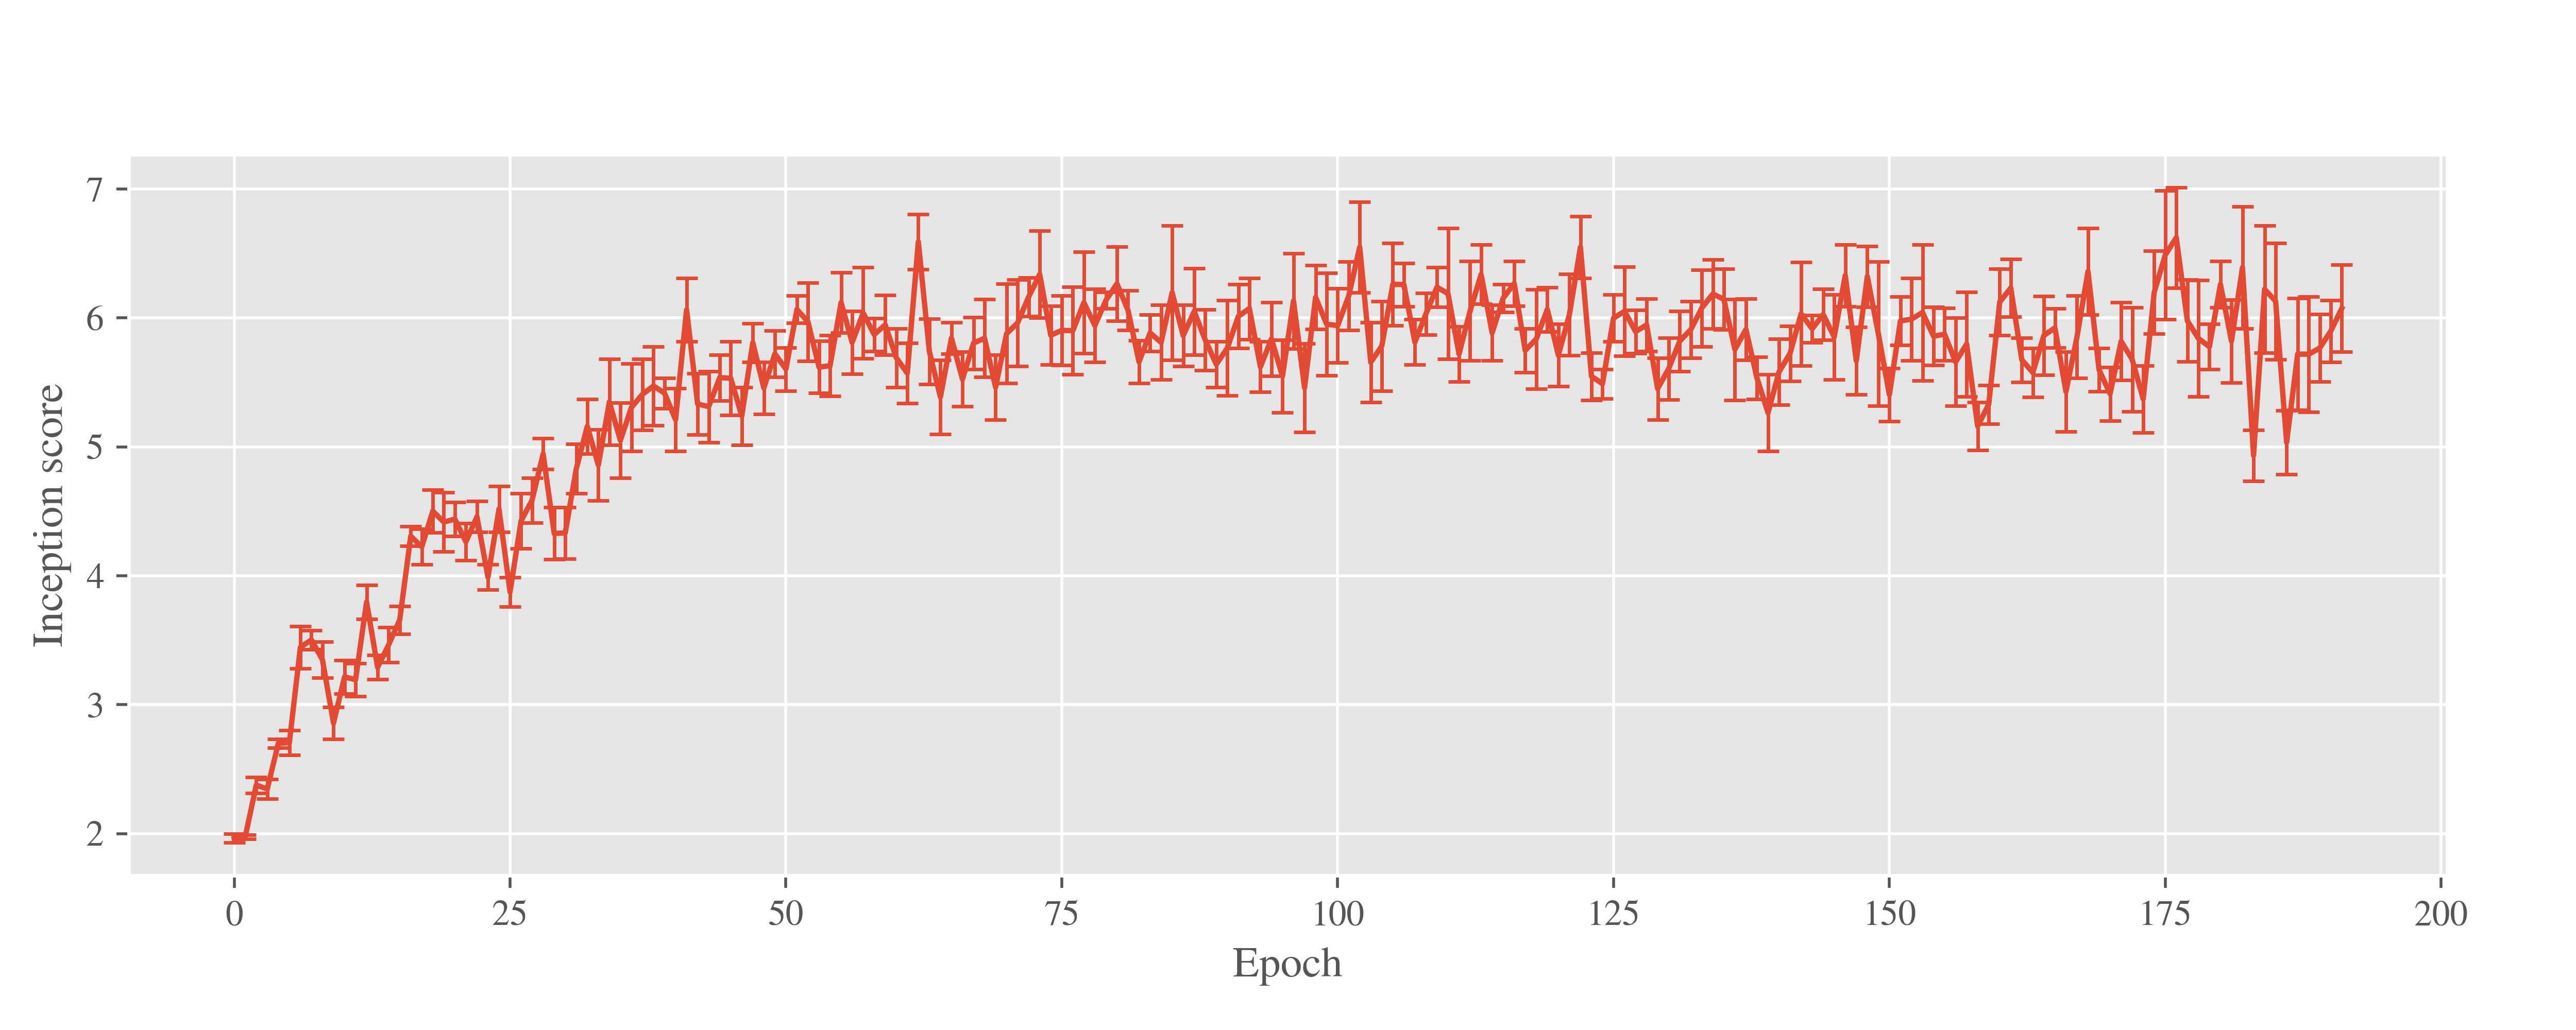
\includegraphics[width=\textwidth]{../code/results/figures/dcgan_cifar10_is.png}
		\caption{Inception score}
		\label{fig:exp-dcgan-is}
    \end{subfigure}
    \begin{subfigure}[t]{0.49\textwidth}
        \centering
        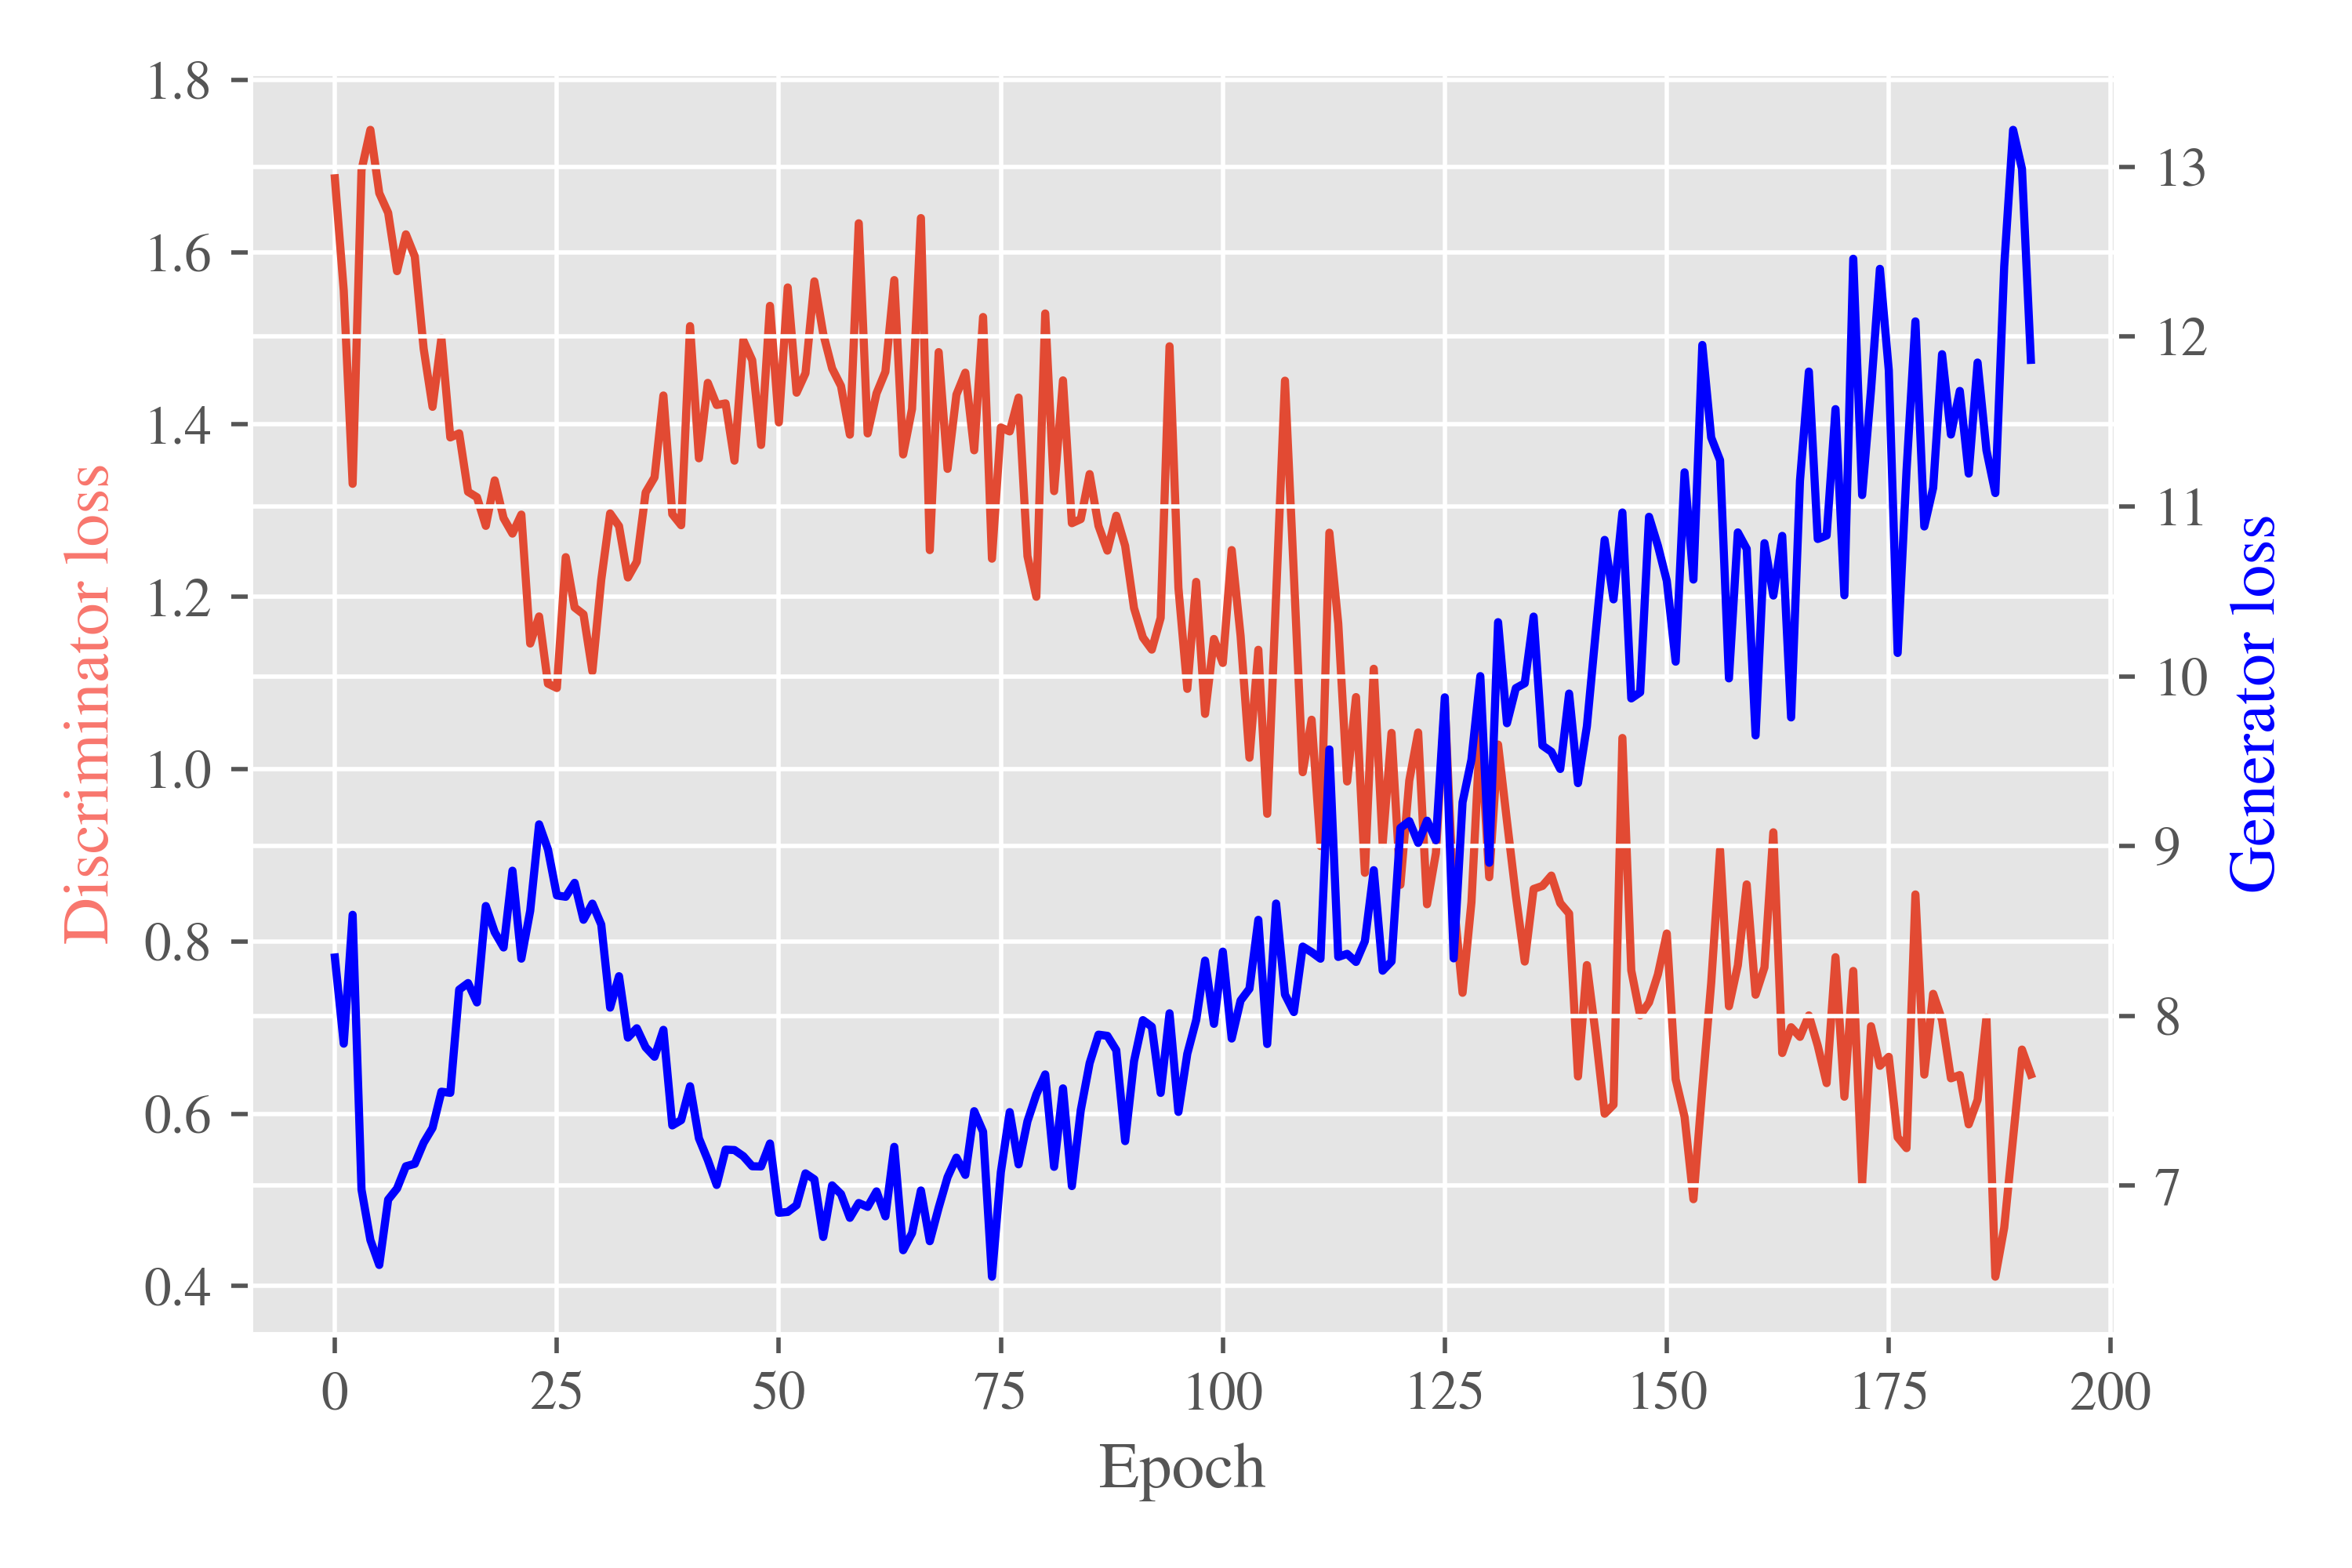
\includegraphics[width=\textwidth]{../code/results/figures/dcgan_cifar10_losses.png}
		\caption{Losses}
		\label{fig:exp-dcgan-losses}
    \end{subfigure}
    \caption{DCGAN - training on CIFAR10 over 190 epochs.}
\end{figure}
We conduct a visual inspection of the generated images and observe that many of them look alike, if not identical. This is a common phenomenon called mode collapse, in which the generator fails to learn the complete multimodal structure of the target data distribution and rather learns a subset of modes, allowing it to trick the discriminator but not to reproduce the target data distribution.
\subsection{SN-DCGAN}
\label{sec:exp-sndcgan}
We implement the spectral normalization layer and use on the discriminator of the DCGAN used in the previous section. We present the evolution of the inception score and losses in Figures \ref{fig:exp-sndcgan-is} and \ref{fig:exp-sndcgan-losses}, respectively.
   
% is
\begin{figure}[h]
\centering
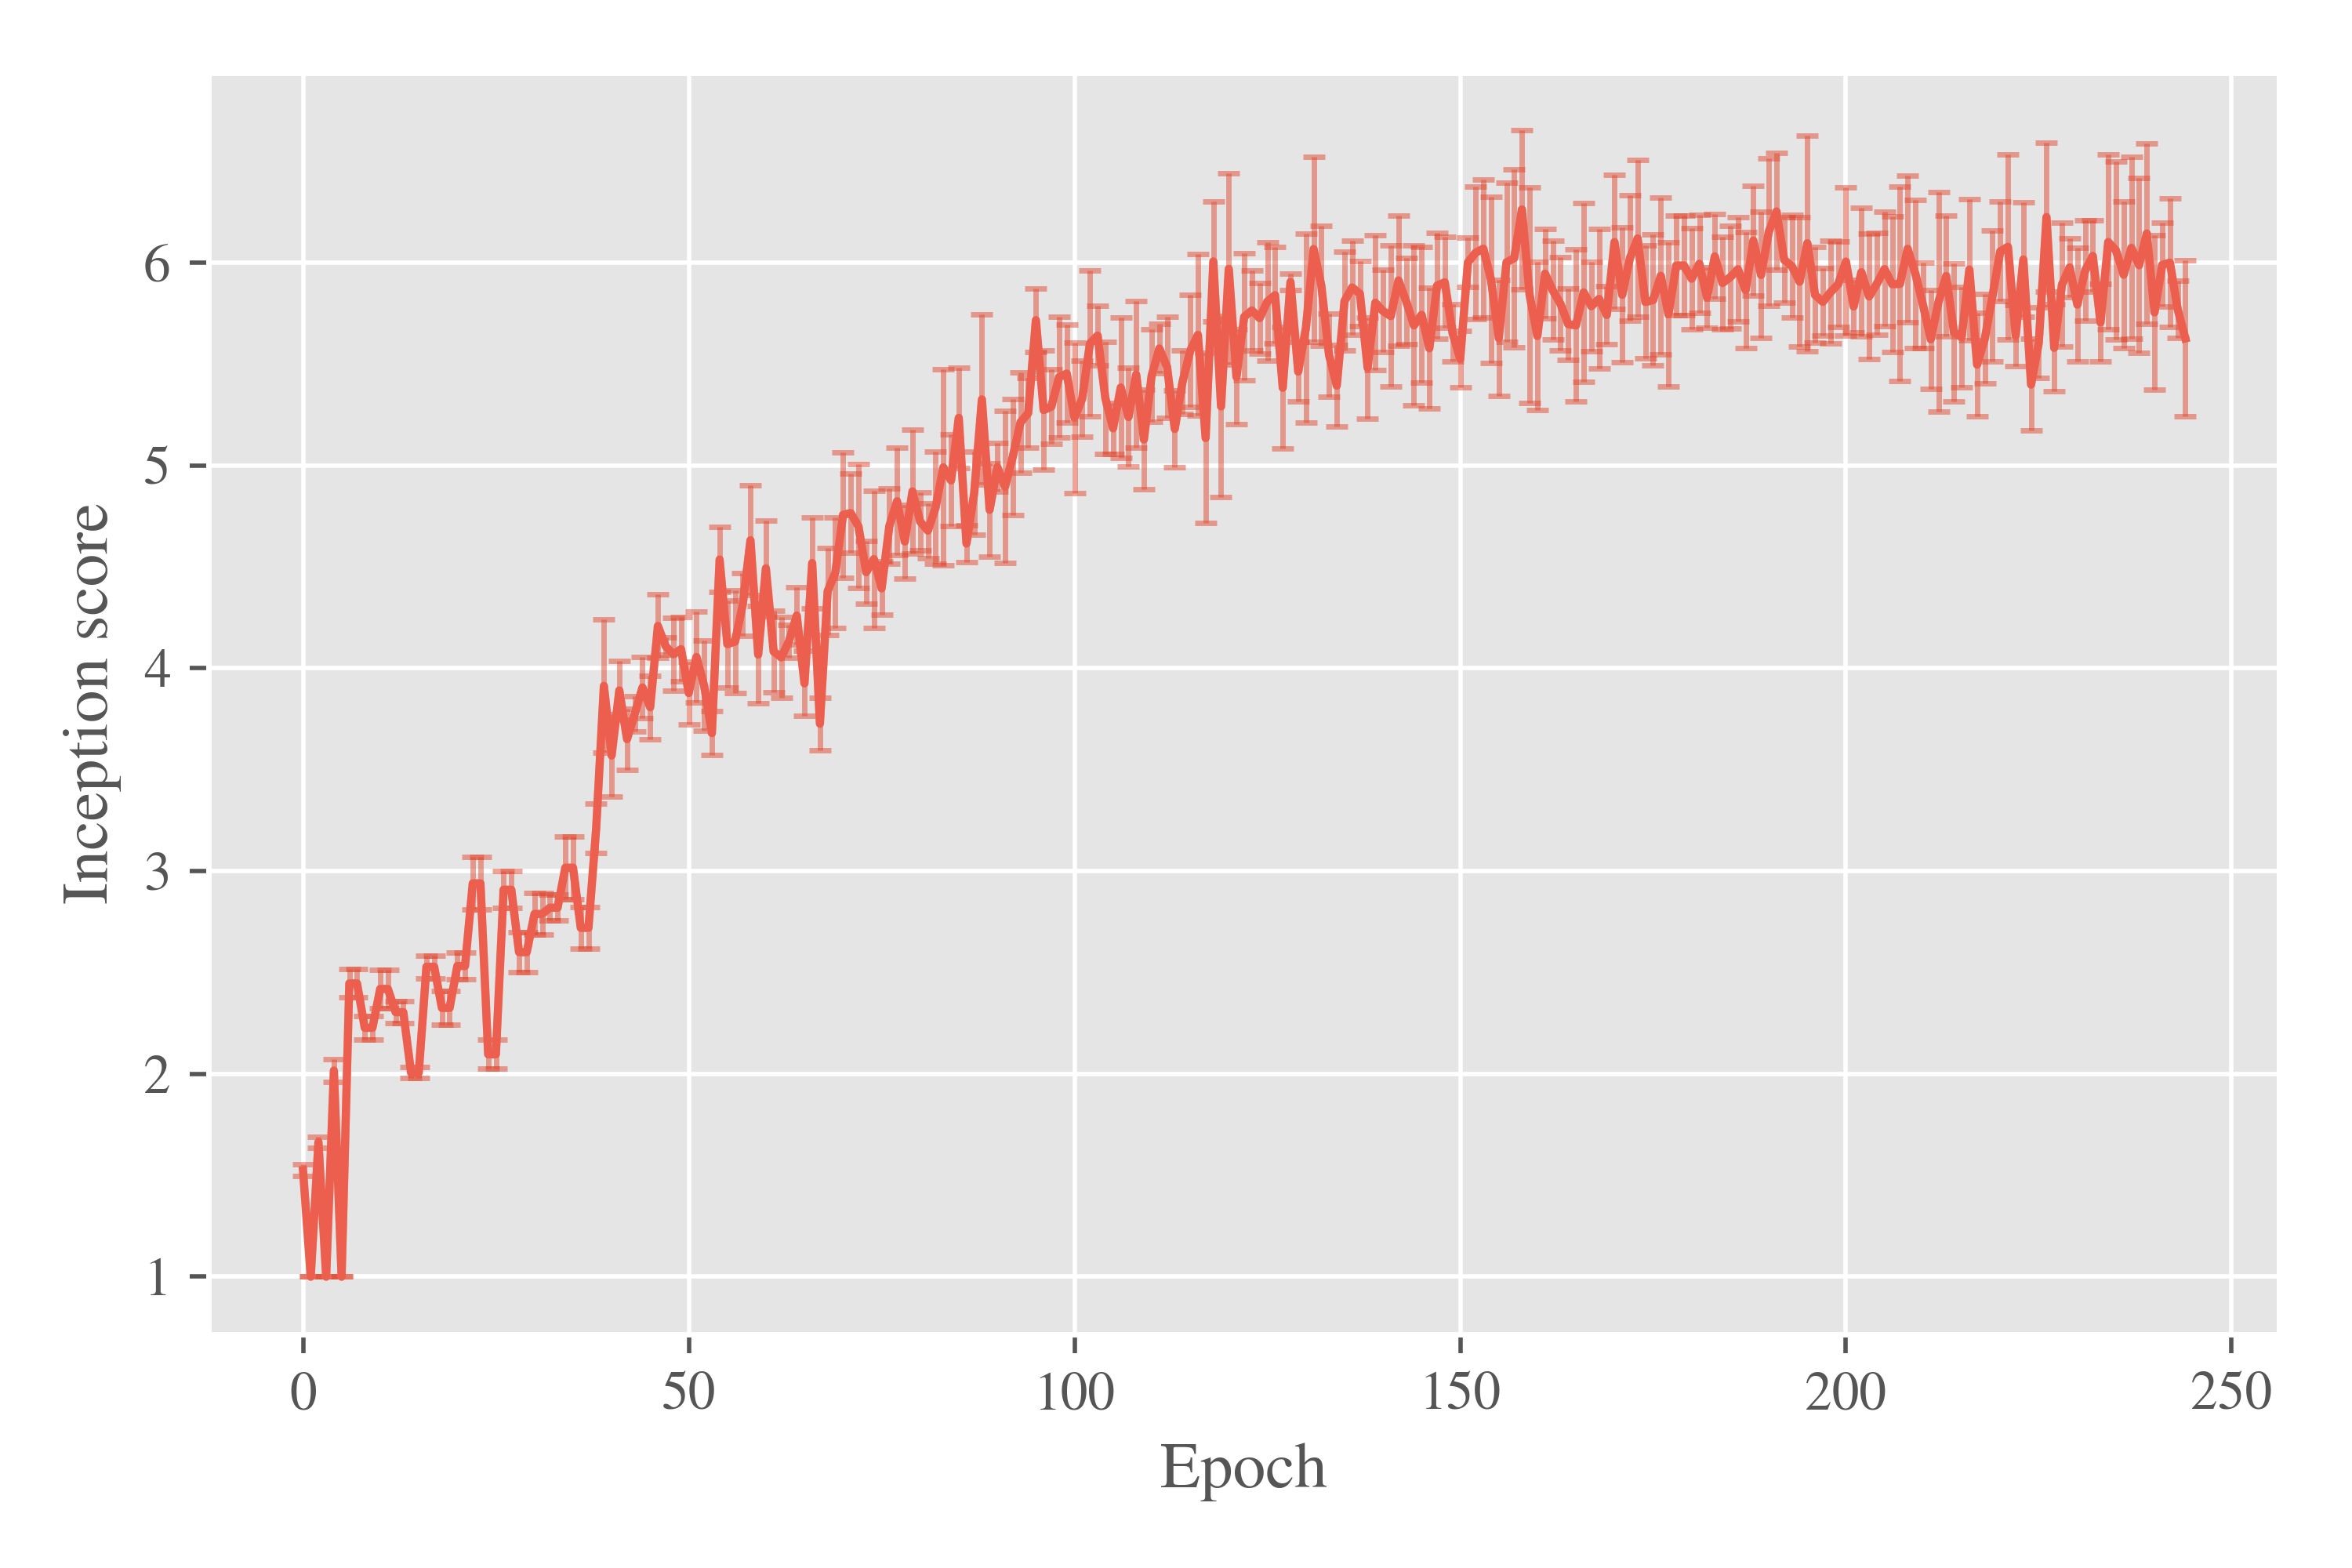
\includegraphics[width=\textwidth]{../code/results/figures/sndcgan_cifar10_is.png}
\caption{SN-DCGAN - Inception score, training on cifar10 over ~250 epochs}
\label{fig:exp-sndcgan-is}
\end{figure}
We don't notice any significant improvement on the mean of the inception score after convergence. However, the average standard deviation is reduced compared to that of the DCGAN without spectral normalization, depicted in Figure \ref{fig:exp-dcgan-is}.
% losses
\begin{figure}[h]
\centering
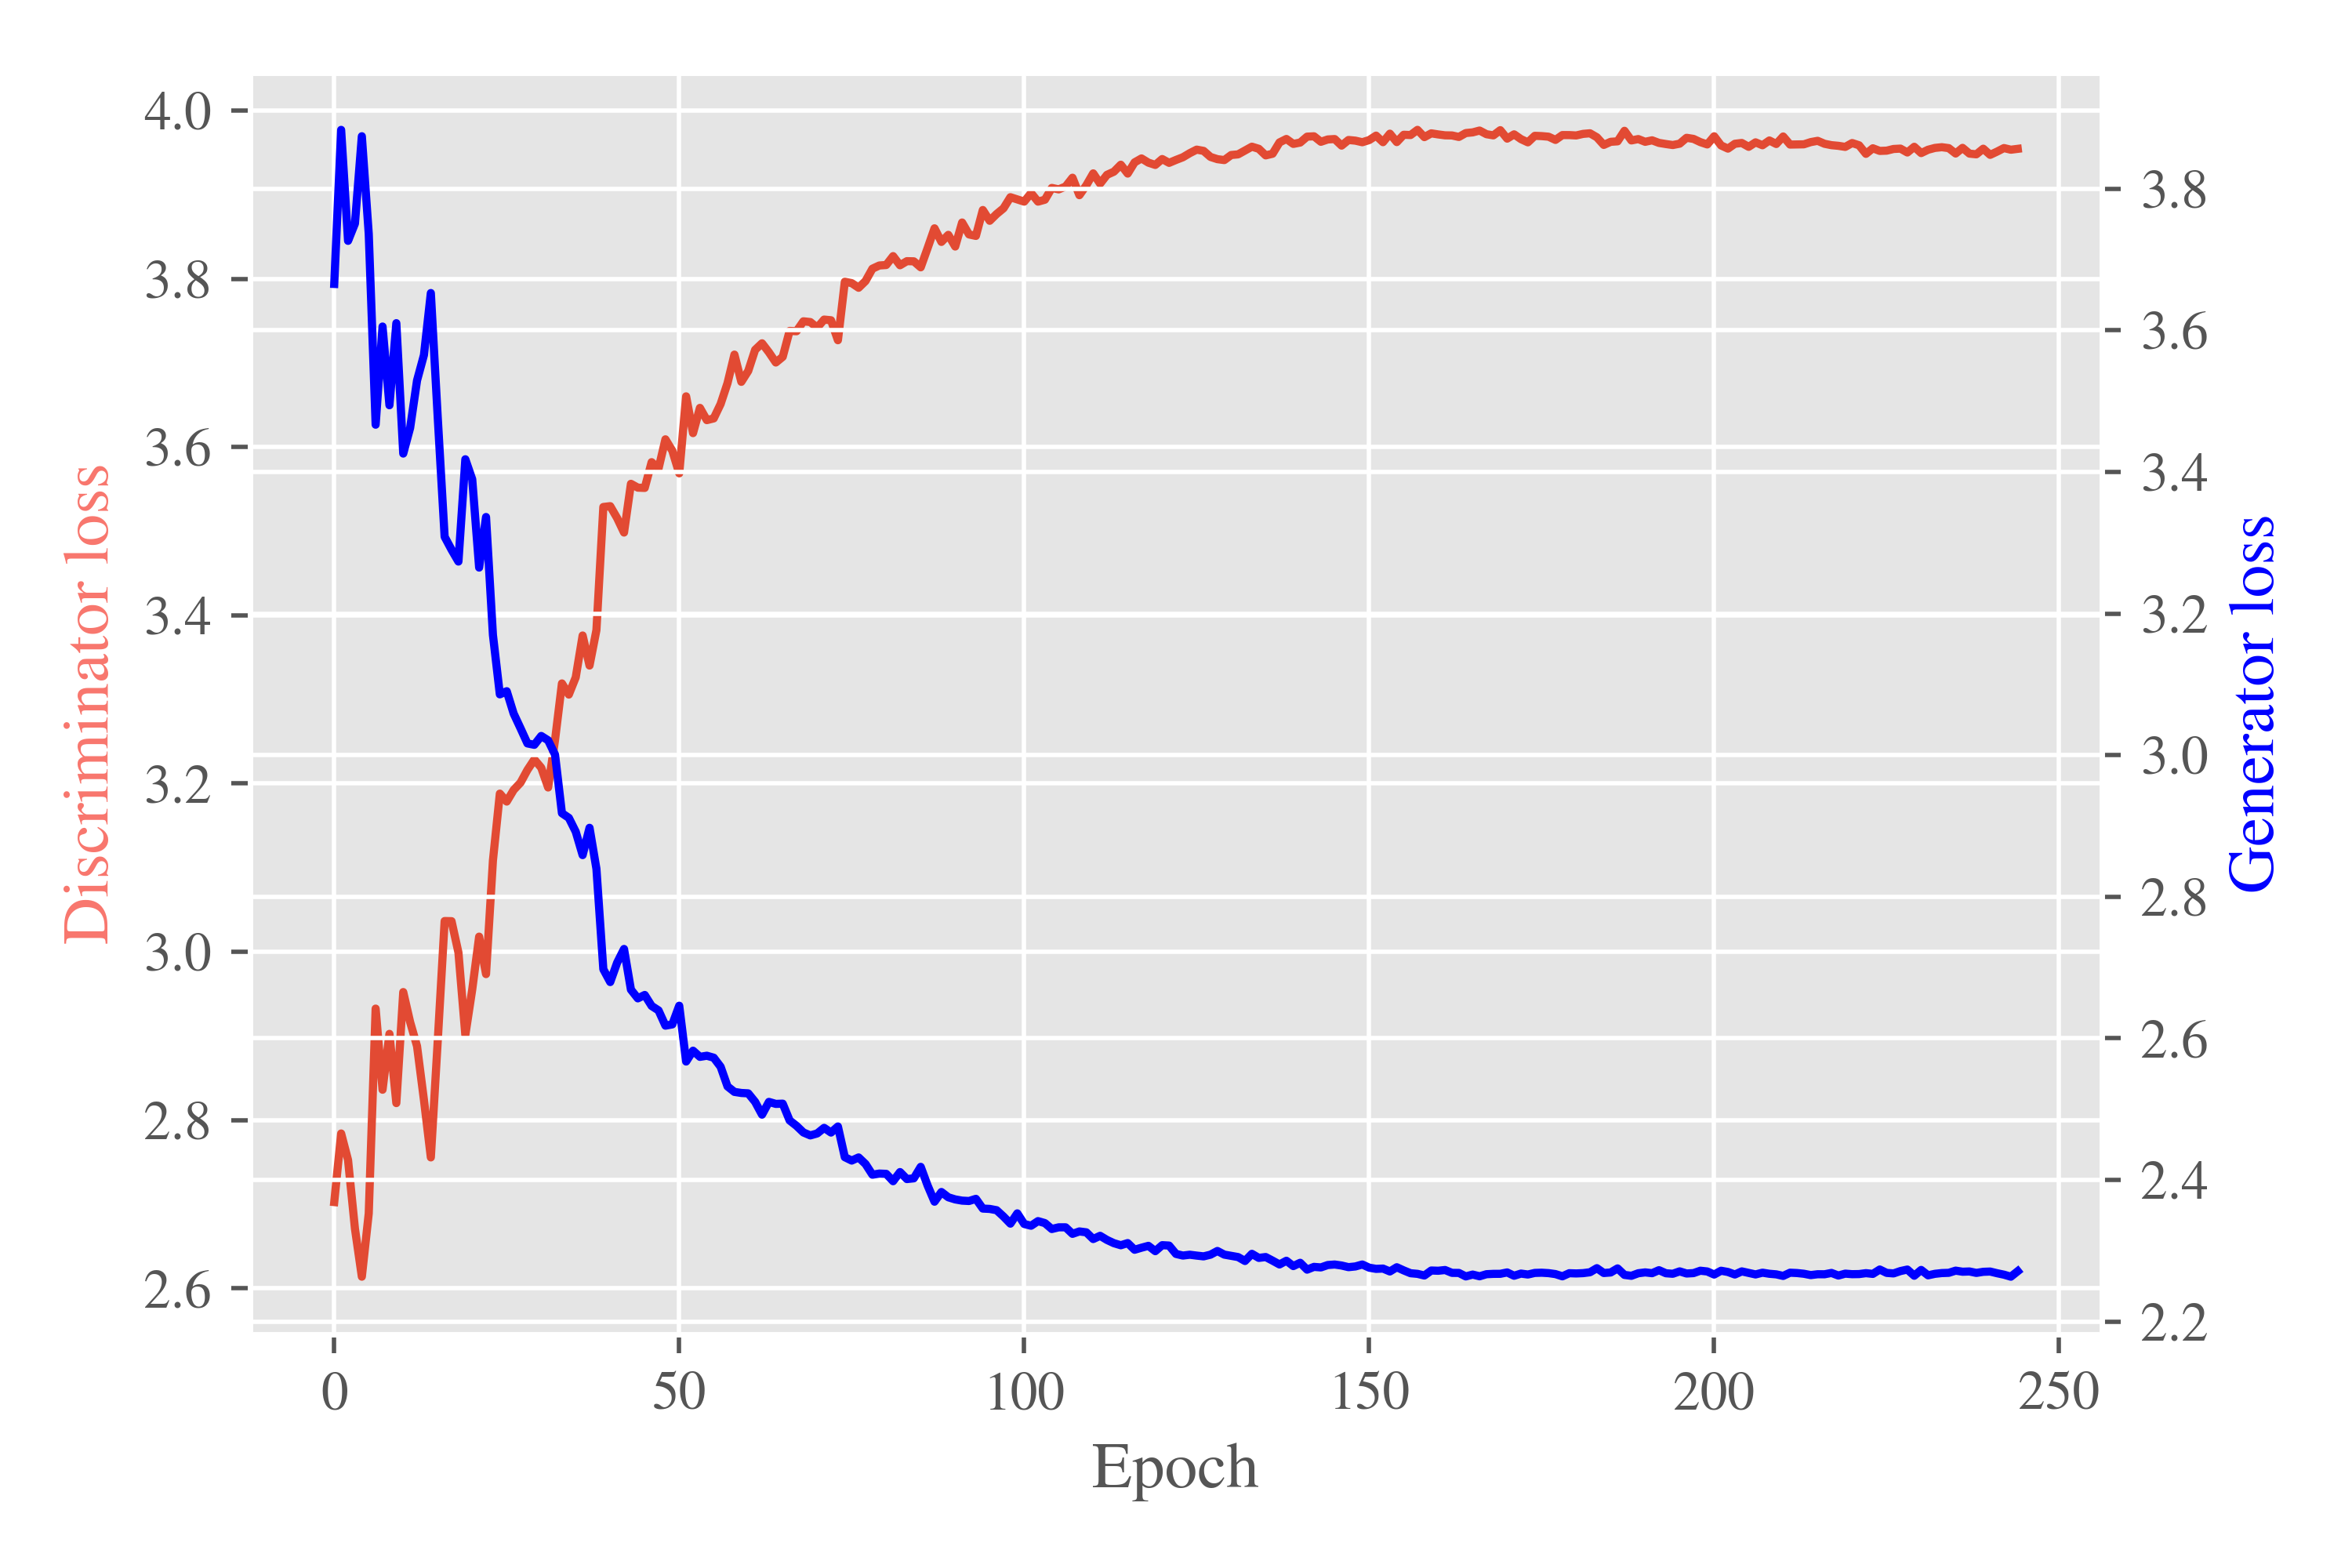
\includegraphics[width=\textwidth]{../code/results/figures/sndcgan_cifar10_losses.png}
\caption{SN-DCGAN - Losses training on cifar10 over ~250 epochs.}
\label{fig:exp-sndcgan-losses}
\end{figure}
In Figure \ref{fig:exp-dcgan-losses}, we observe that both losses are much smoother with spectral normalization. This is the desired result; the original intent of the paper on spectral normalization was to provide a solution to stabilize the training of GANs \cite{miyato2018spectral}. 
\subsection{W-DCGAN}
\label{sec:exp-w-dcgan}
We present the evolution of the Inception score and losses in Figures \ref{fig:exp-w-dcgan-is} and \ref{fig:exp-w-dcgan-losses}, respectively. We did not expect to a get good performance using this setup since we did not implement any method enforcing the Lipschitz continuity of the discriminator functions, which is required by WGAN. These results coincide with our expectations.
   
\begin{figure}[H]
    \centering
    \begin{subfigure}[t]{0.49\textwidth}
        \centering
		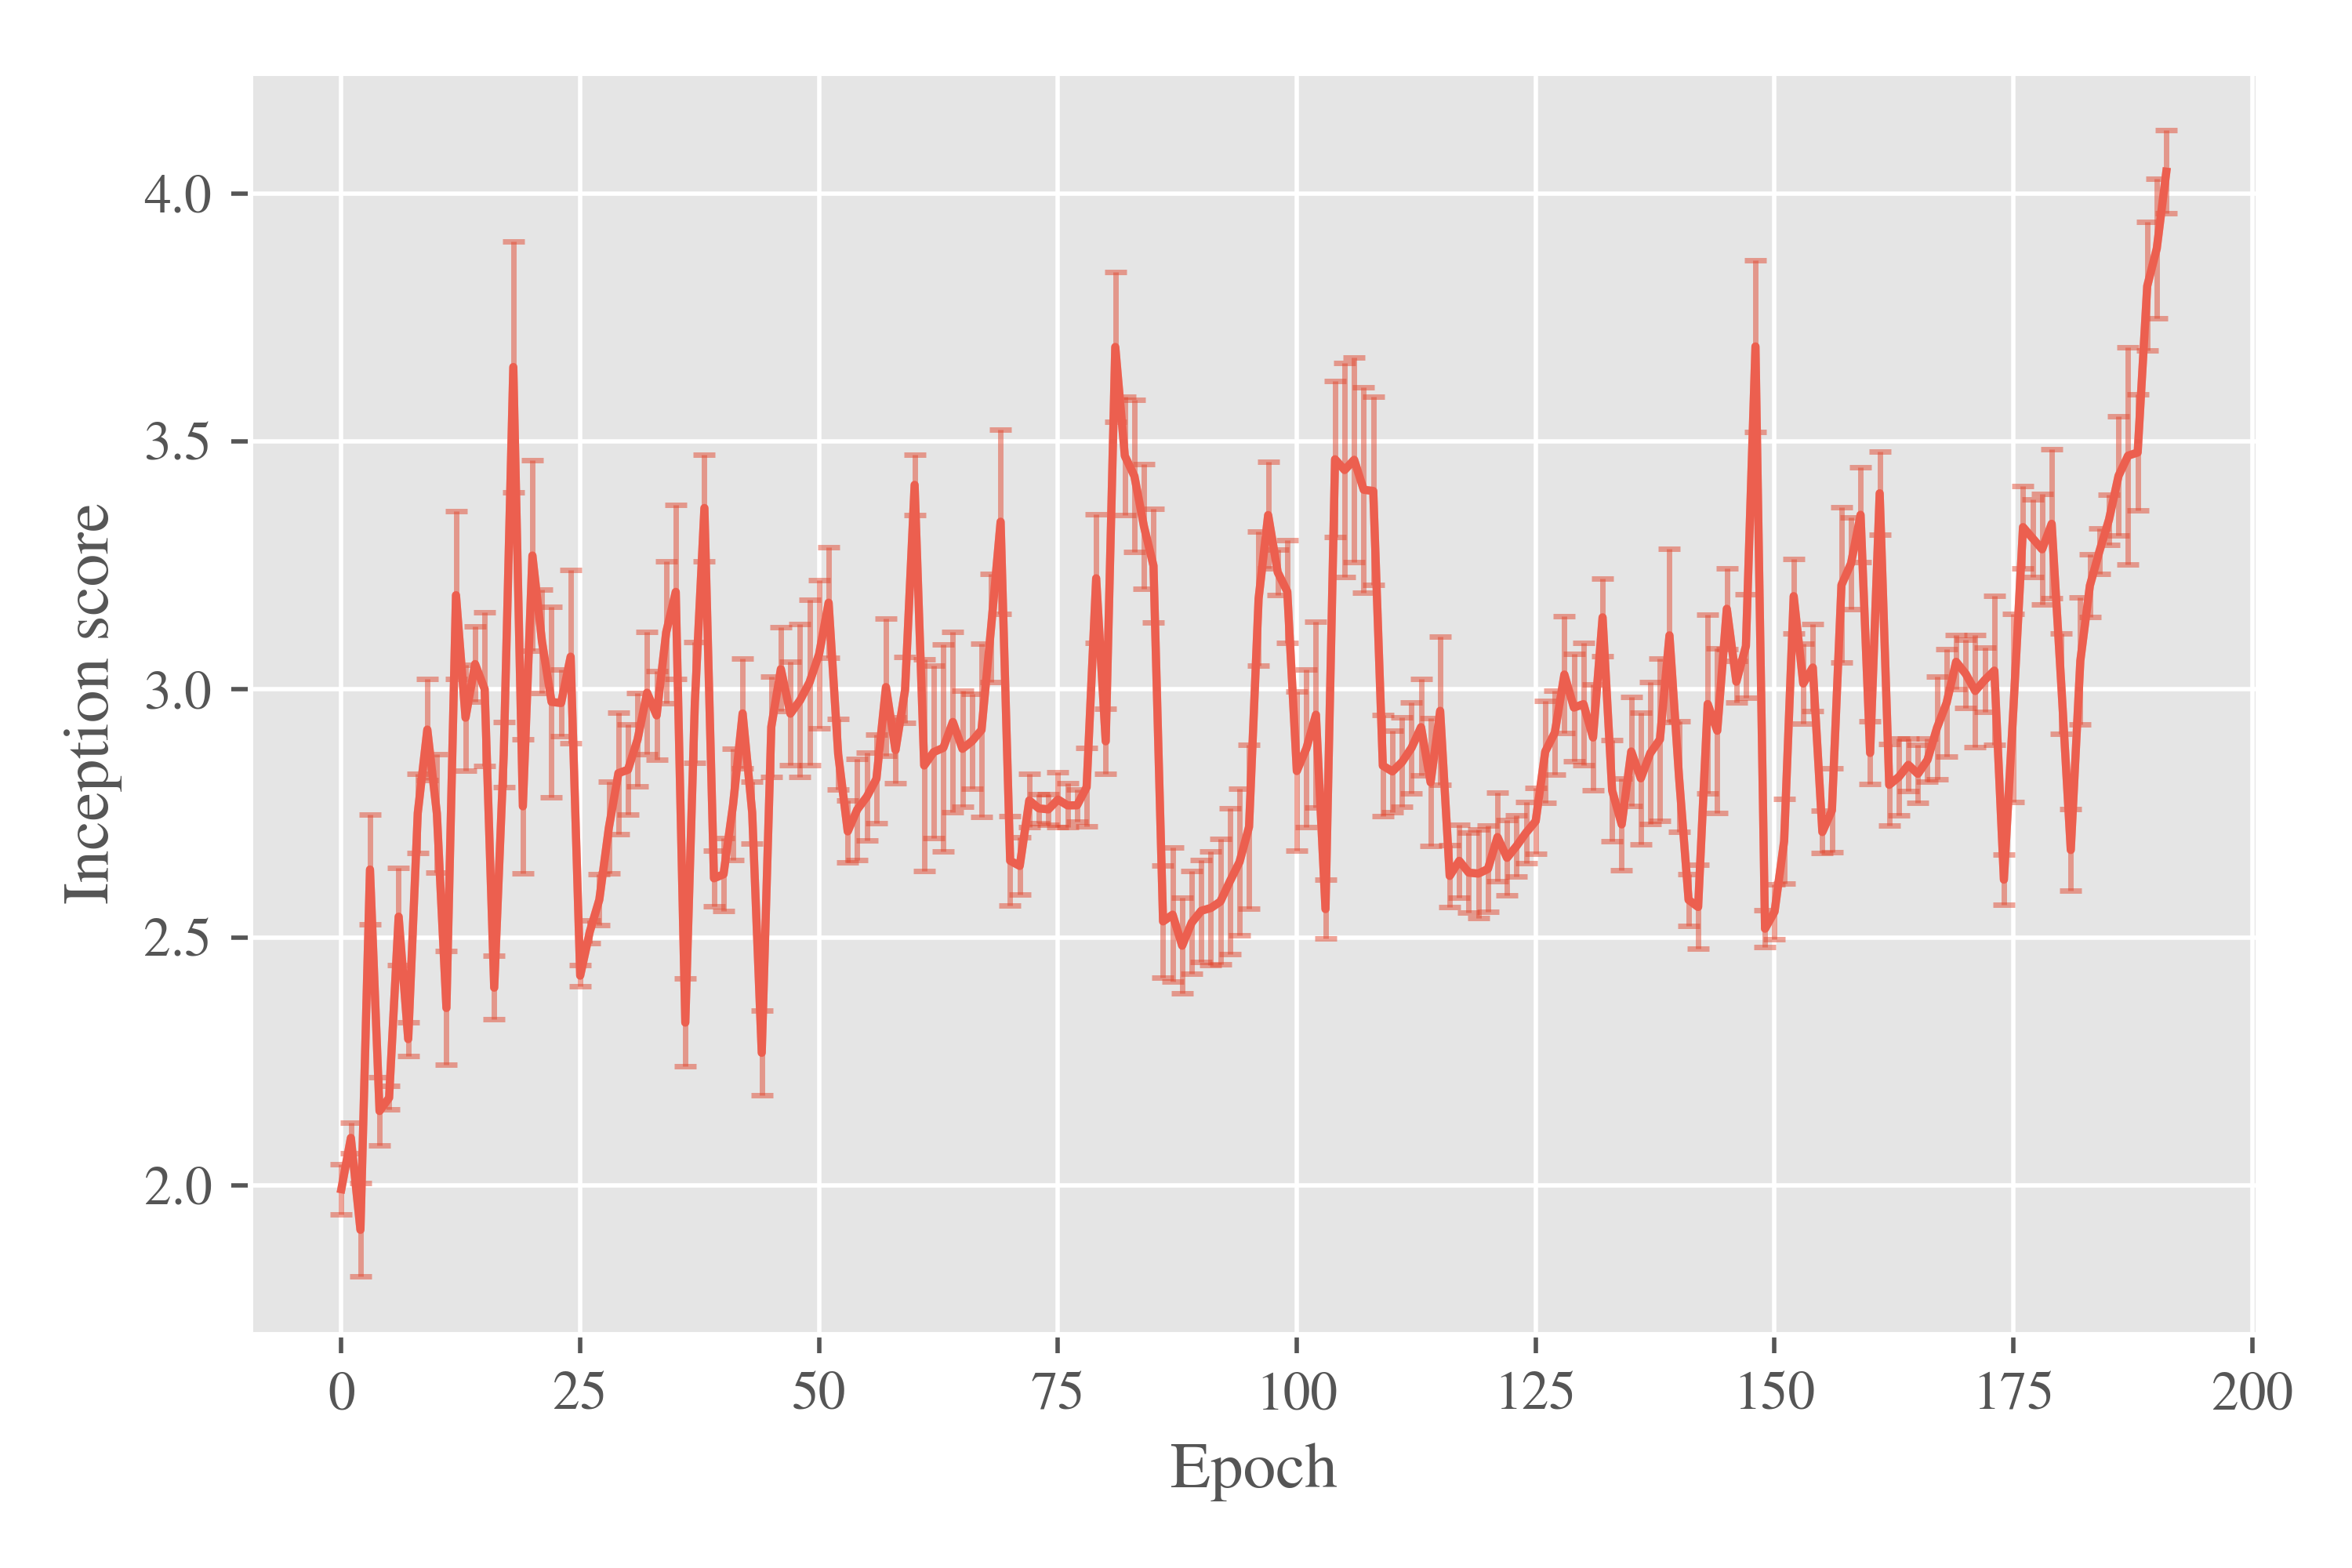
\includegraphics[width=\textwidth]{../code/results/figures/w-dcgan_cifar10_is.png}
		\caption{Inception score\\~}
		\label{fig:exp-w-dcgan-is}
    \end{subfigure}
    \begin{subfigure}[t]{0.49\textwidth}
        \centering
        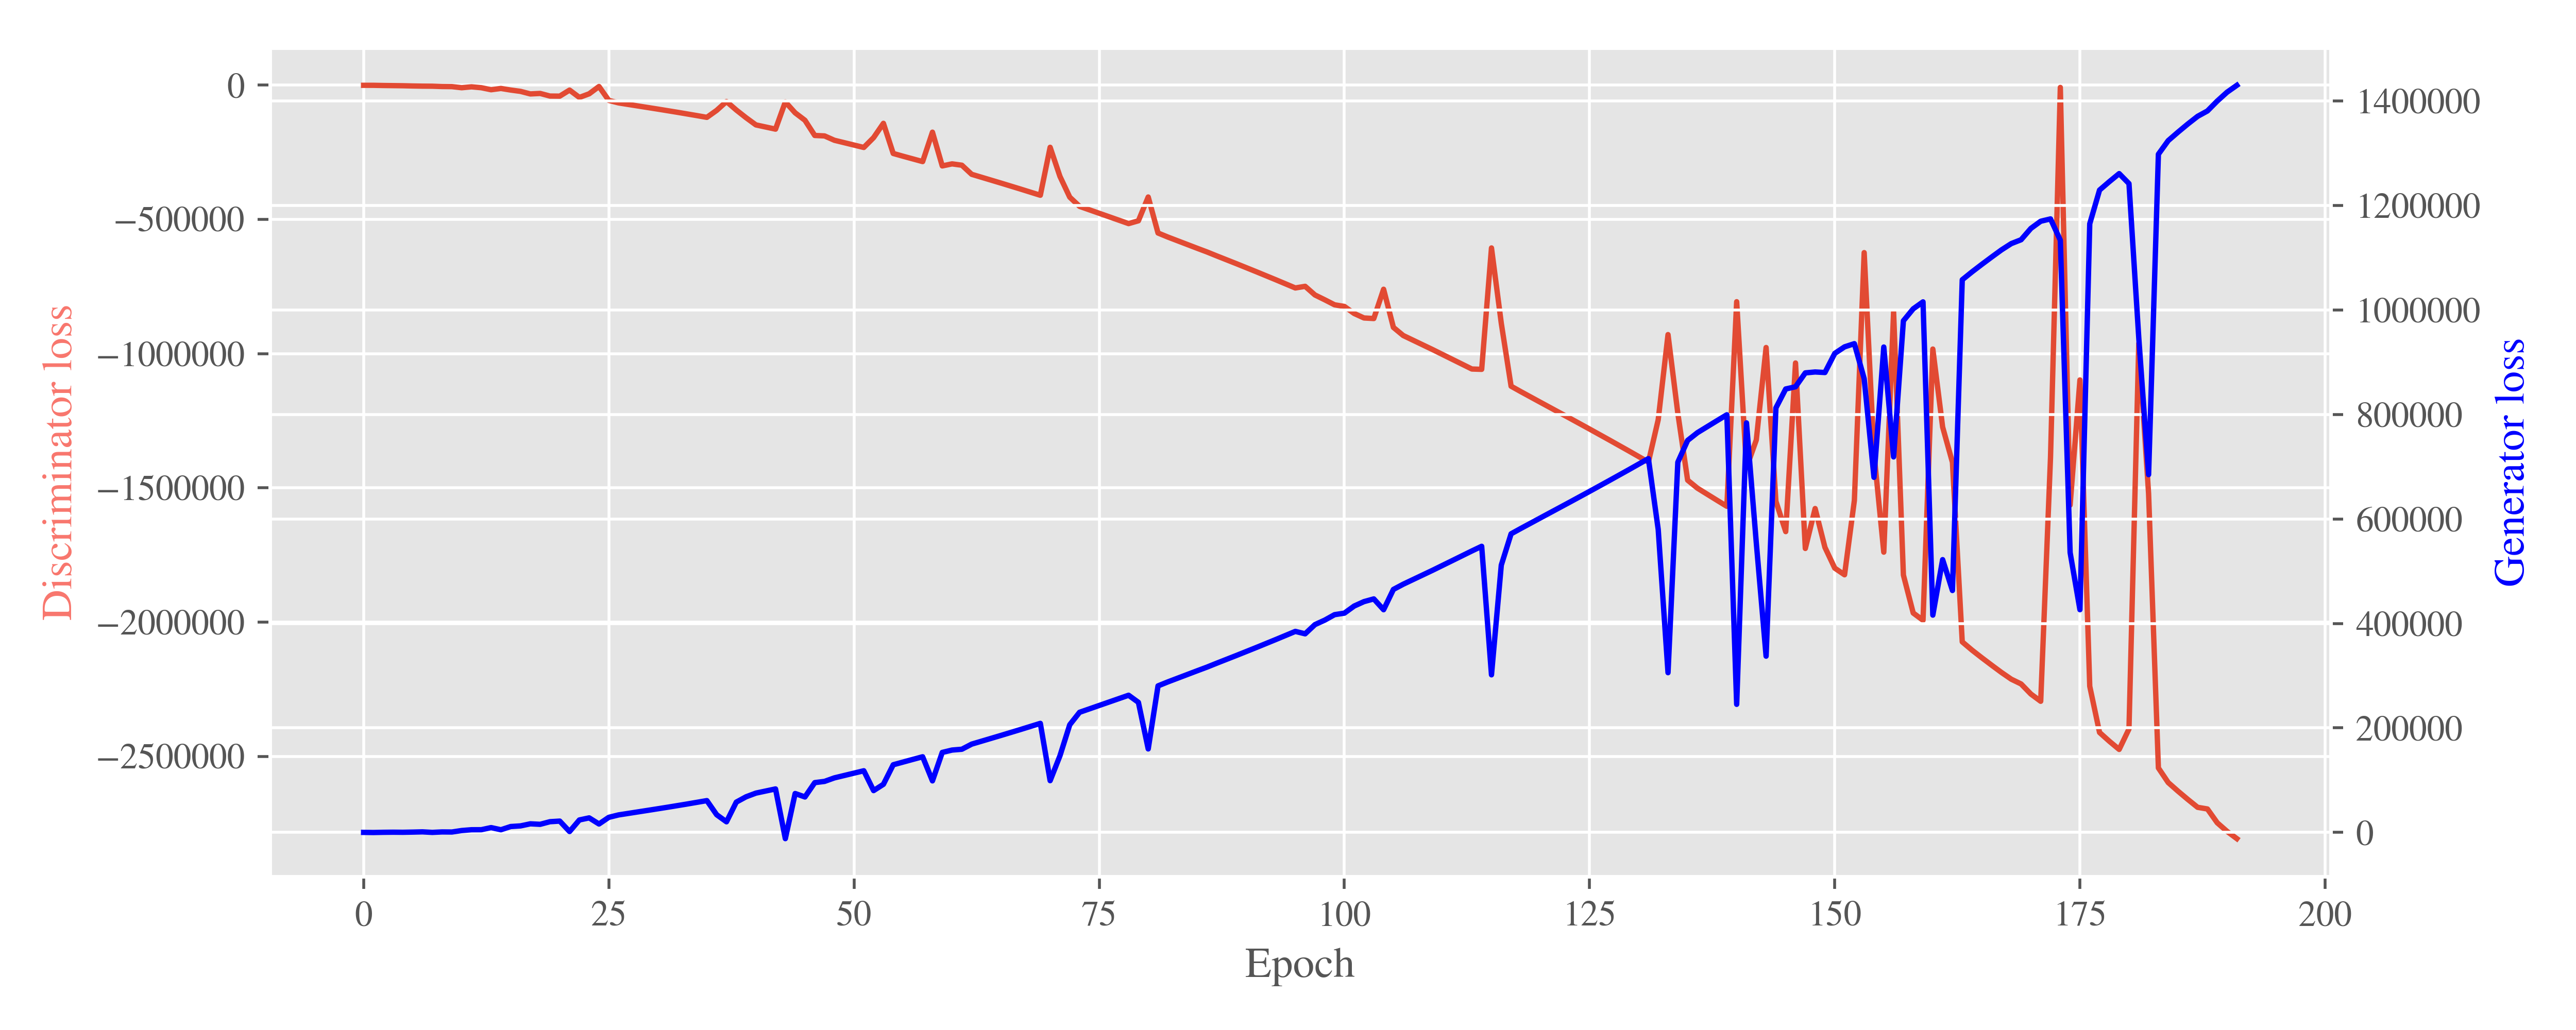
\includegraphics[width=\textwidth]{../code/results/figures/w-dcgan_cifar10_losses.png}
		\caption{Losses\\~}
		\label{fig:exp-w-dcgan-losses}
    \end{subfigure}
    \caption{W-DCGAN - training on CIFAR10 over 200 epochs.}
\end{figure}

%We observe that both losses are much smoother with spectral normalization. This is the desired result; the original intent of the paper on spectral normalization was to provide a solution to stabilize the training of GANs \cite{miyato2018spectral}. By visual inspection of the generated images we observe a significant reduce in mode collapse and a noticeable improvement of image quality. This did however not result in a significant Inception score improvement.
\subsection{W-WC-DCGAN}
\label{sec:exp-w-wc-dcgan}
We implement weight clipping (WC) on top of the W-DCGAN from the previous section. As stated before, the authors of WGAN state that this method is a far from ideal way to ensure a norm on the gradients. However, we still expect it to outperform the W-DCGAN. We present the evolution of the Inception score and losses in Figures \ref{fig:exp-w-wc-dcgan-is} and \ref{fig:exp-w-wc-dcgan-losses}, respectively. %
\begin{figure}[H]
    \centering
    \begin{subfigure}[t]{0.49\textwidth}
        \centering
		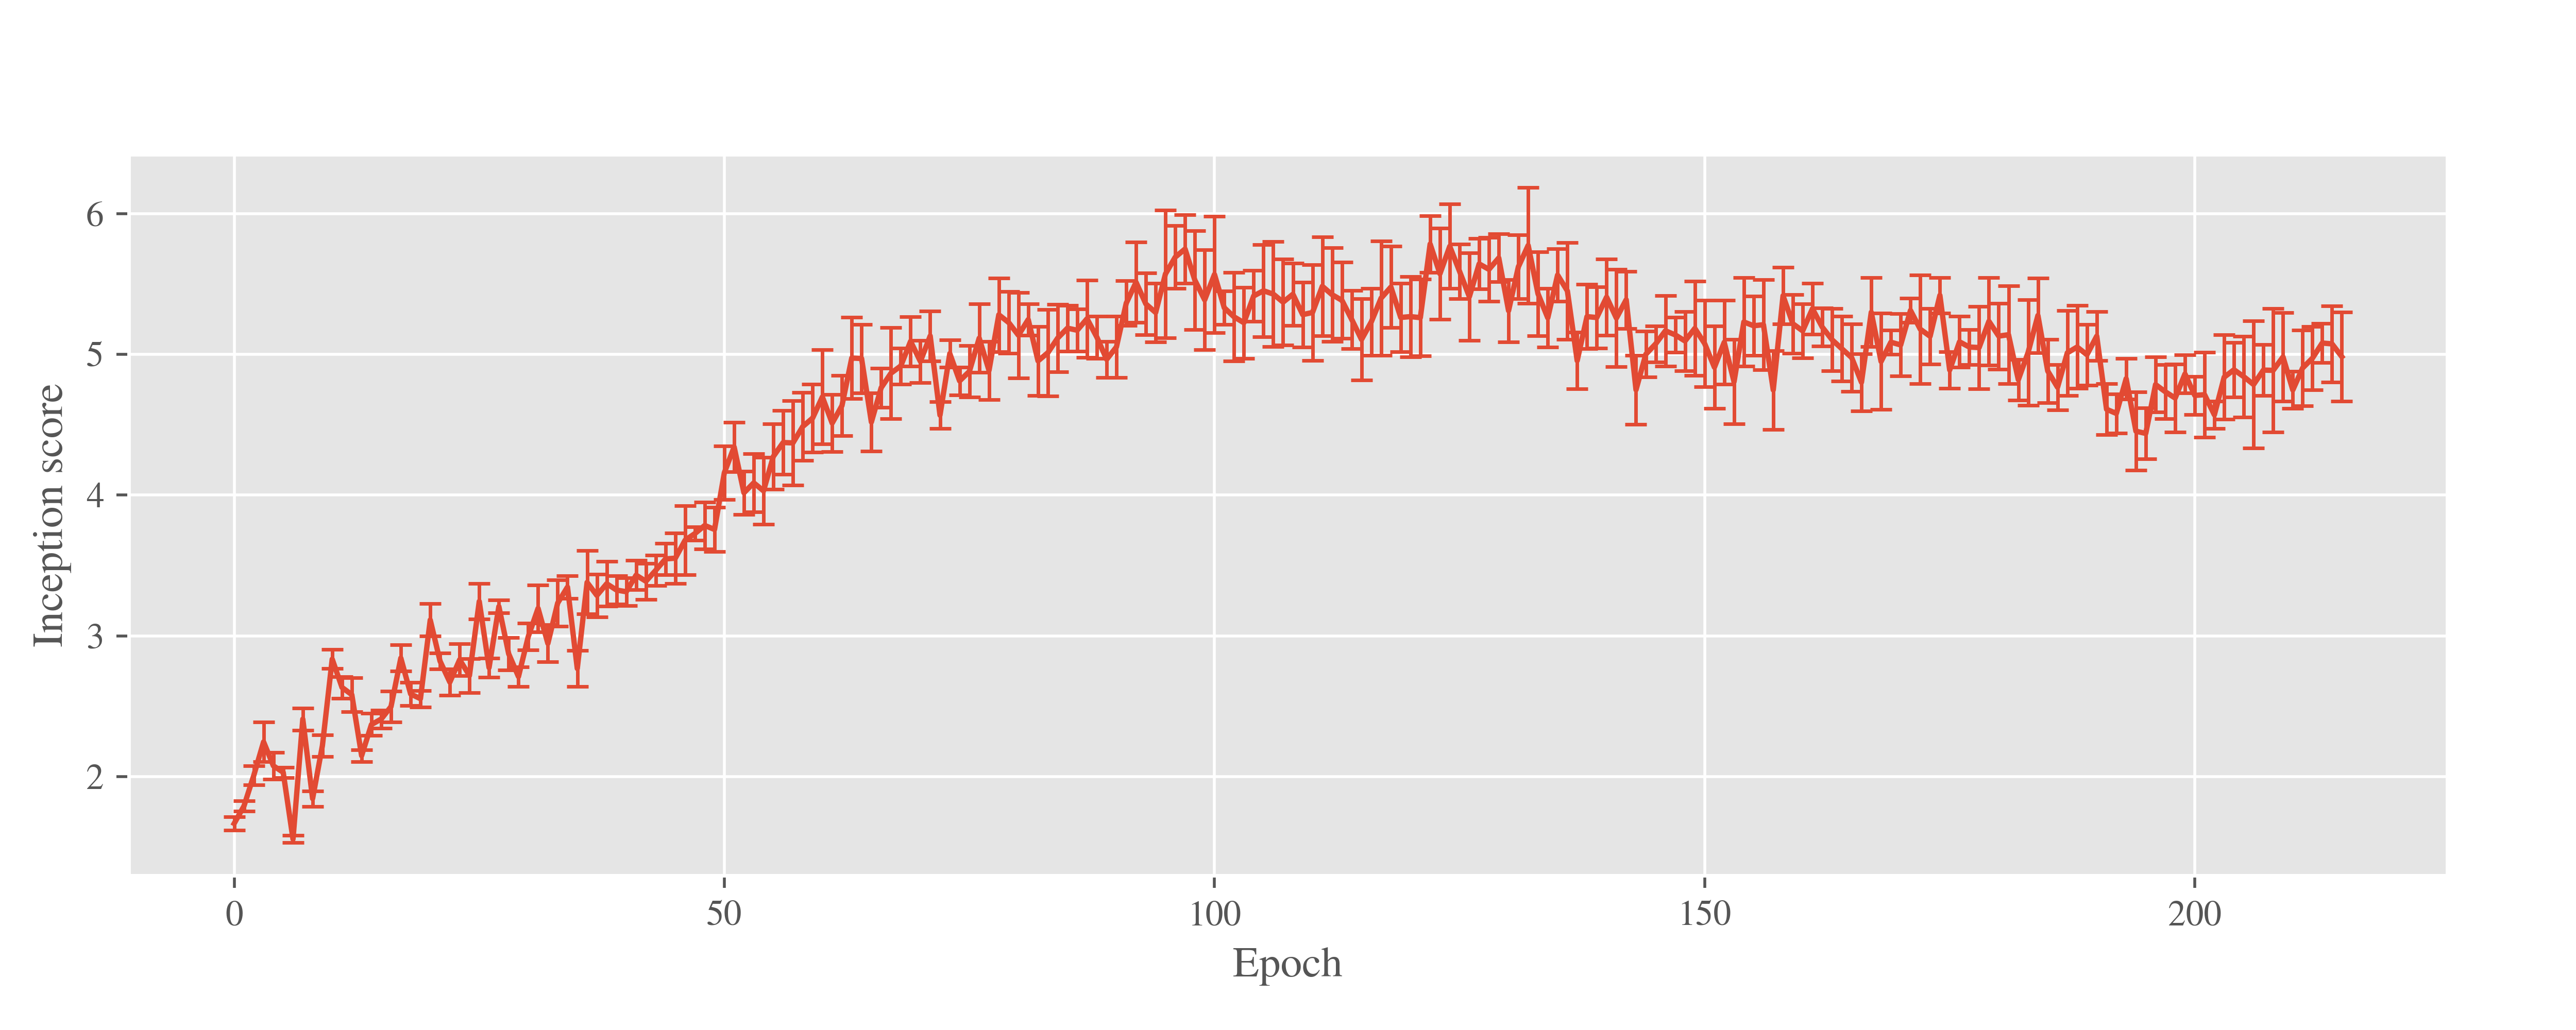
\includegraphics[width=\textwidth]{../code/results/figures/w-wc-dcgan_cifar10_is.png}
		\caption{Inception score\\~}
		\label{fig:exp-w-wc-dcgan-is}
    \end{subfigure}
    \begin{subfigure}[t]{0.49\textwidth}
        \centering
        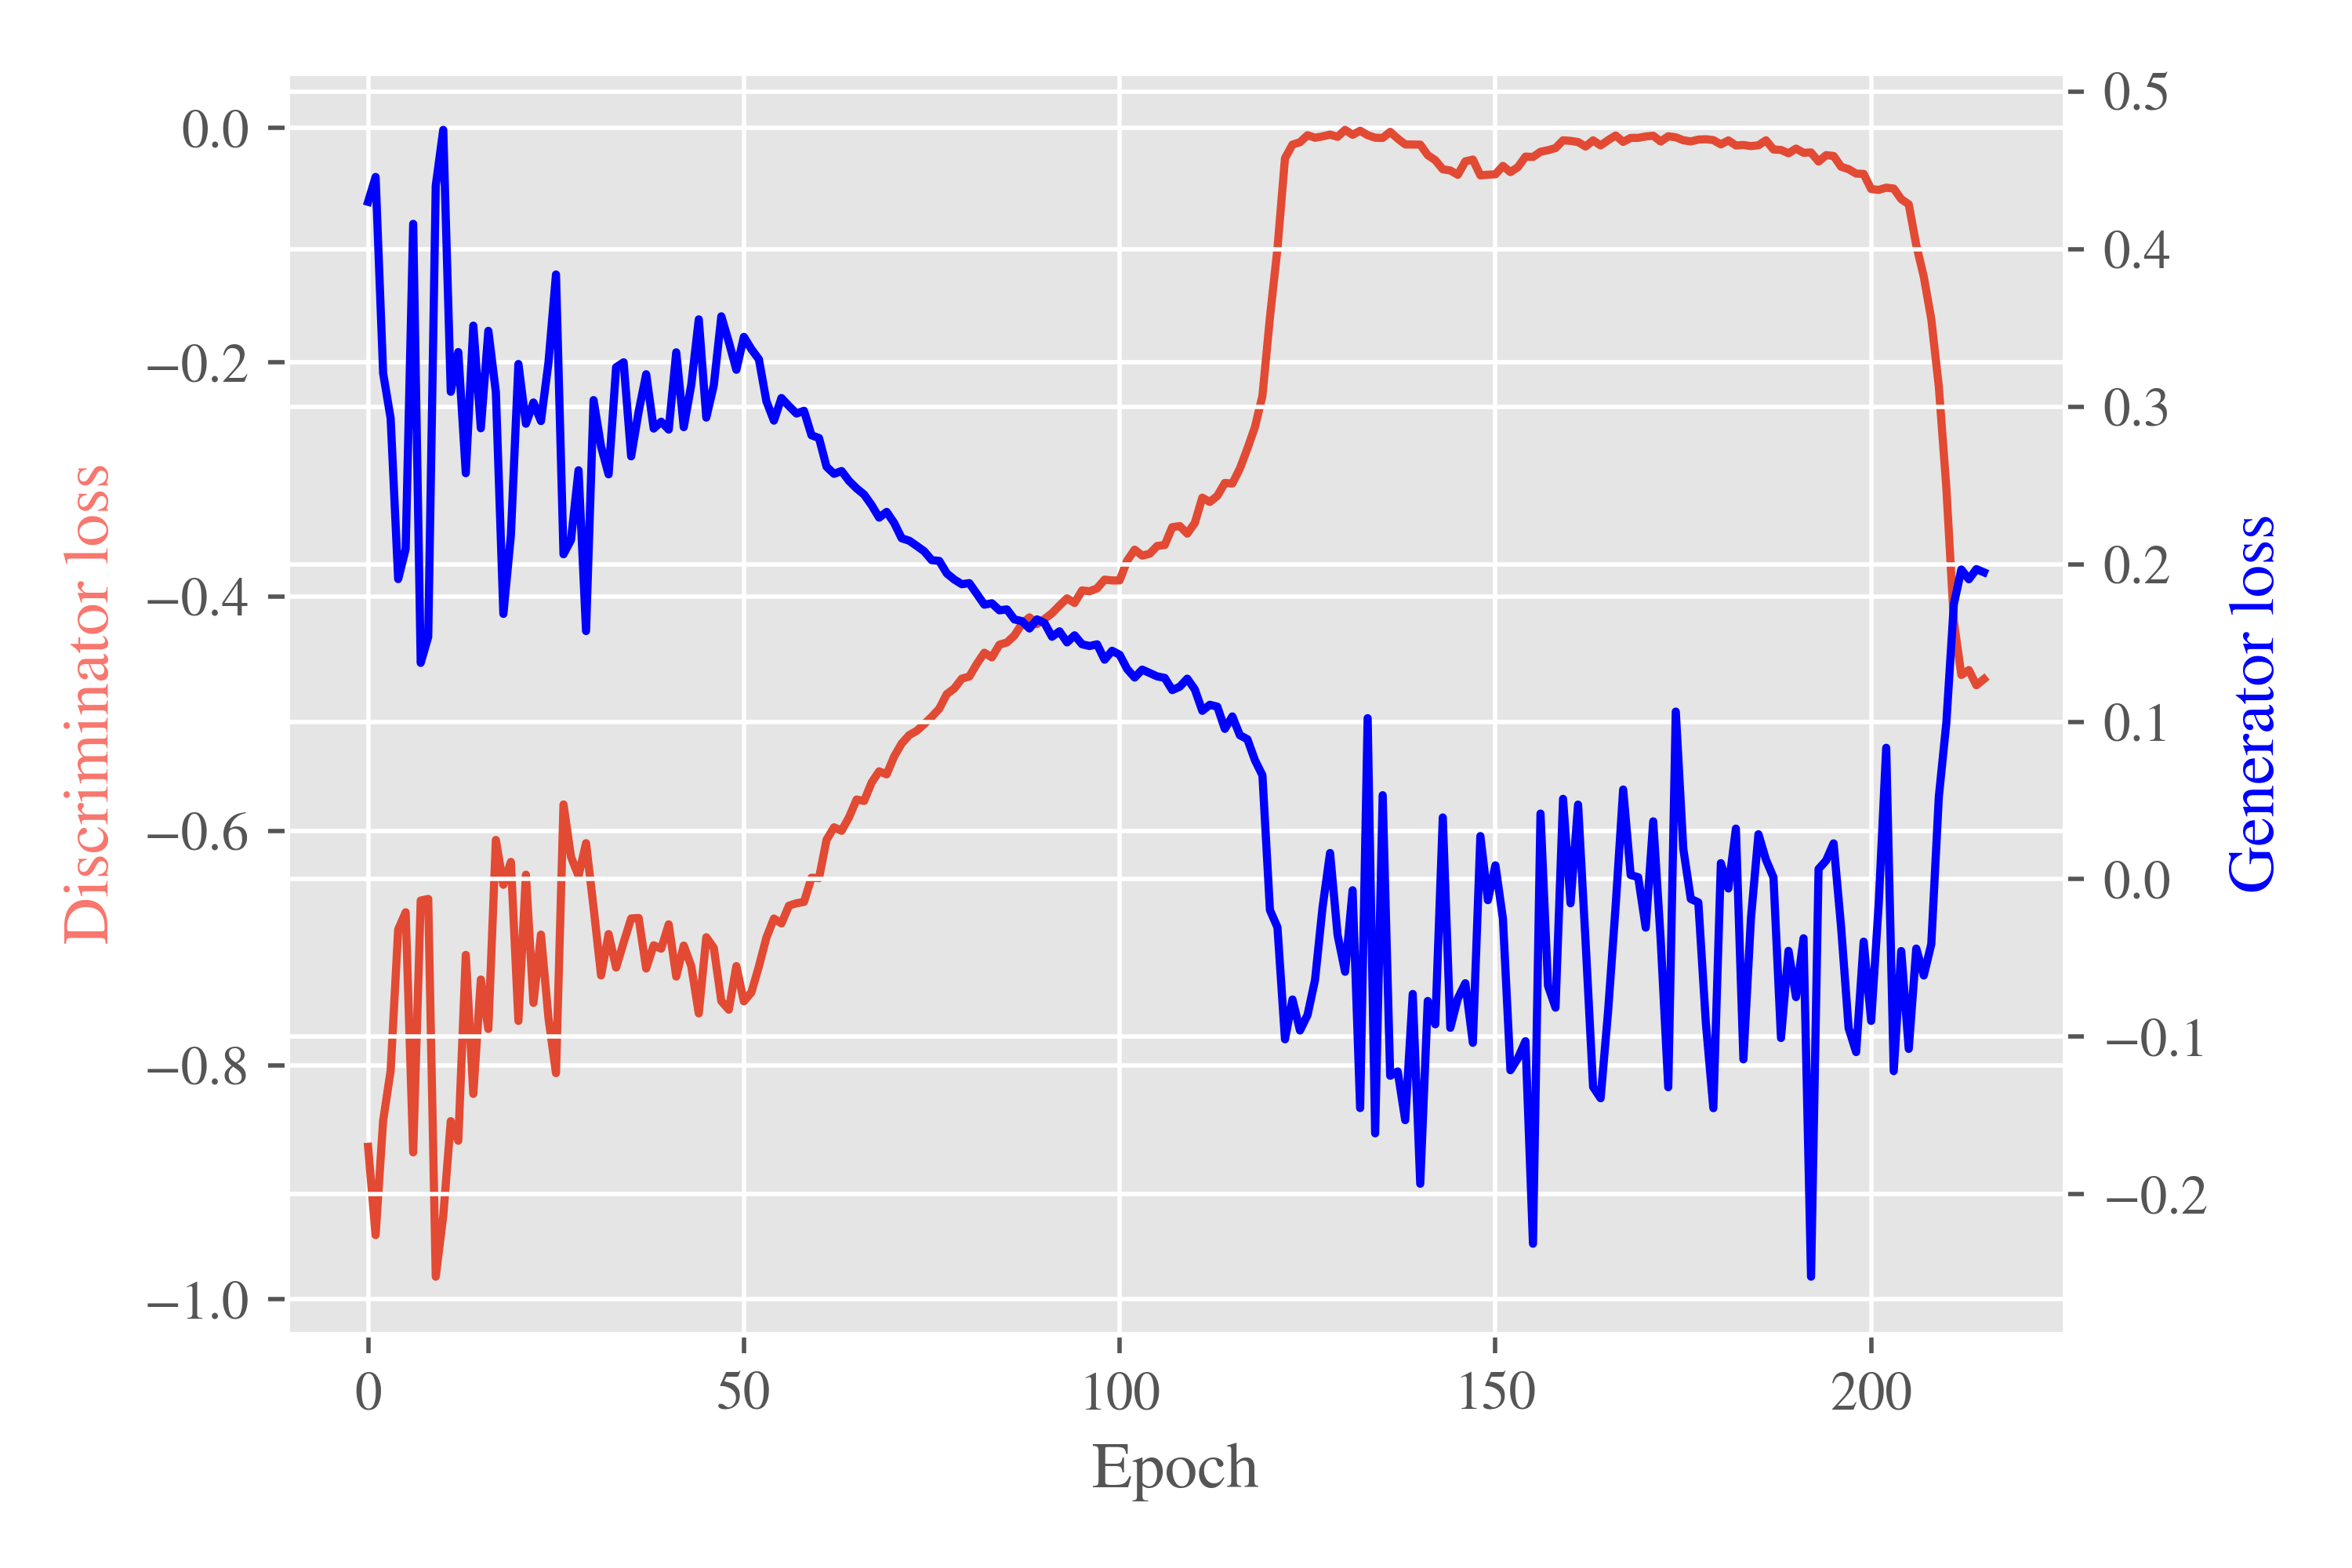
\includegraphics[width=\textwidth]{../code/results/figures/w-wc-dcgan_cifar10_losses.png}
		\caption{Losses\\~}
		\label{fig:exp-w-wc-dcgan-losses}
    \end{subfigure}
    \caption{W-WC-DCGAN - training on CIFAR10 over 200 epochs.}
\end{figure}%
We observe a turbulent climb for the Inception score and an even more chaotic evolution of the losses. Looking at the losses, it seems like the training has two different ``regimes''. We propose an interpretation, even though we cannot be sure of its accuracy. In all experiments, we initialize weights by sampling from a Normal distribution with mean 0 and standard deviation 0.02. Here, we use the recommended clipping value of 0.01 \cite{arjovsky2017wasserstein}. This means that for the first iterations, most weights are systematically clipped, and possibly by a lot. It is easy to think how this would lead to unpredictable or unstable behaviour, seemingly experienced in epochs 0 to 50. Then, we think that weights enter a range that suits the requirements of WGAN, leading to a more stable training phase until epoch 120. After this epoch, the generator seems to enter a new chaotic regime, possibly because the discriminator reached a well performing region where it becomes hard to fool. This problem might be solved with thorough hyper-parameter tuning.
\subsection{W-SN-DCGAN}
\label{sec:exp-wsndcgan}

We present the evolution of the inception score and losses in Figures \ref{fig:exp-wsndcgan-is} and \ref{fig:exp-wsndcgan-losses}, respectively.
   
\begin{figure}[t!]
    \centering
    \begin{subfigure}[t]{0.49\textwidth}
        \centering
		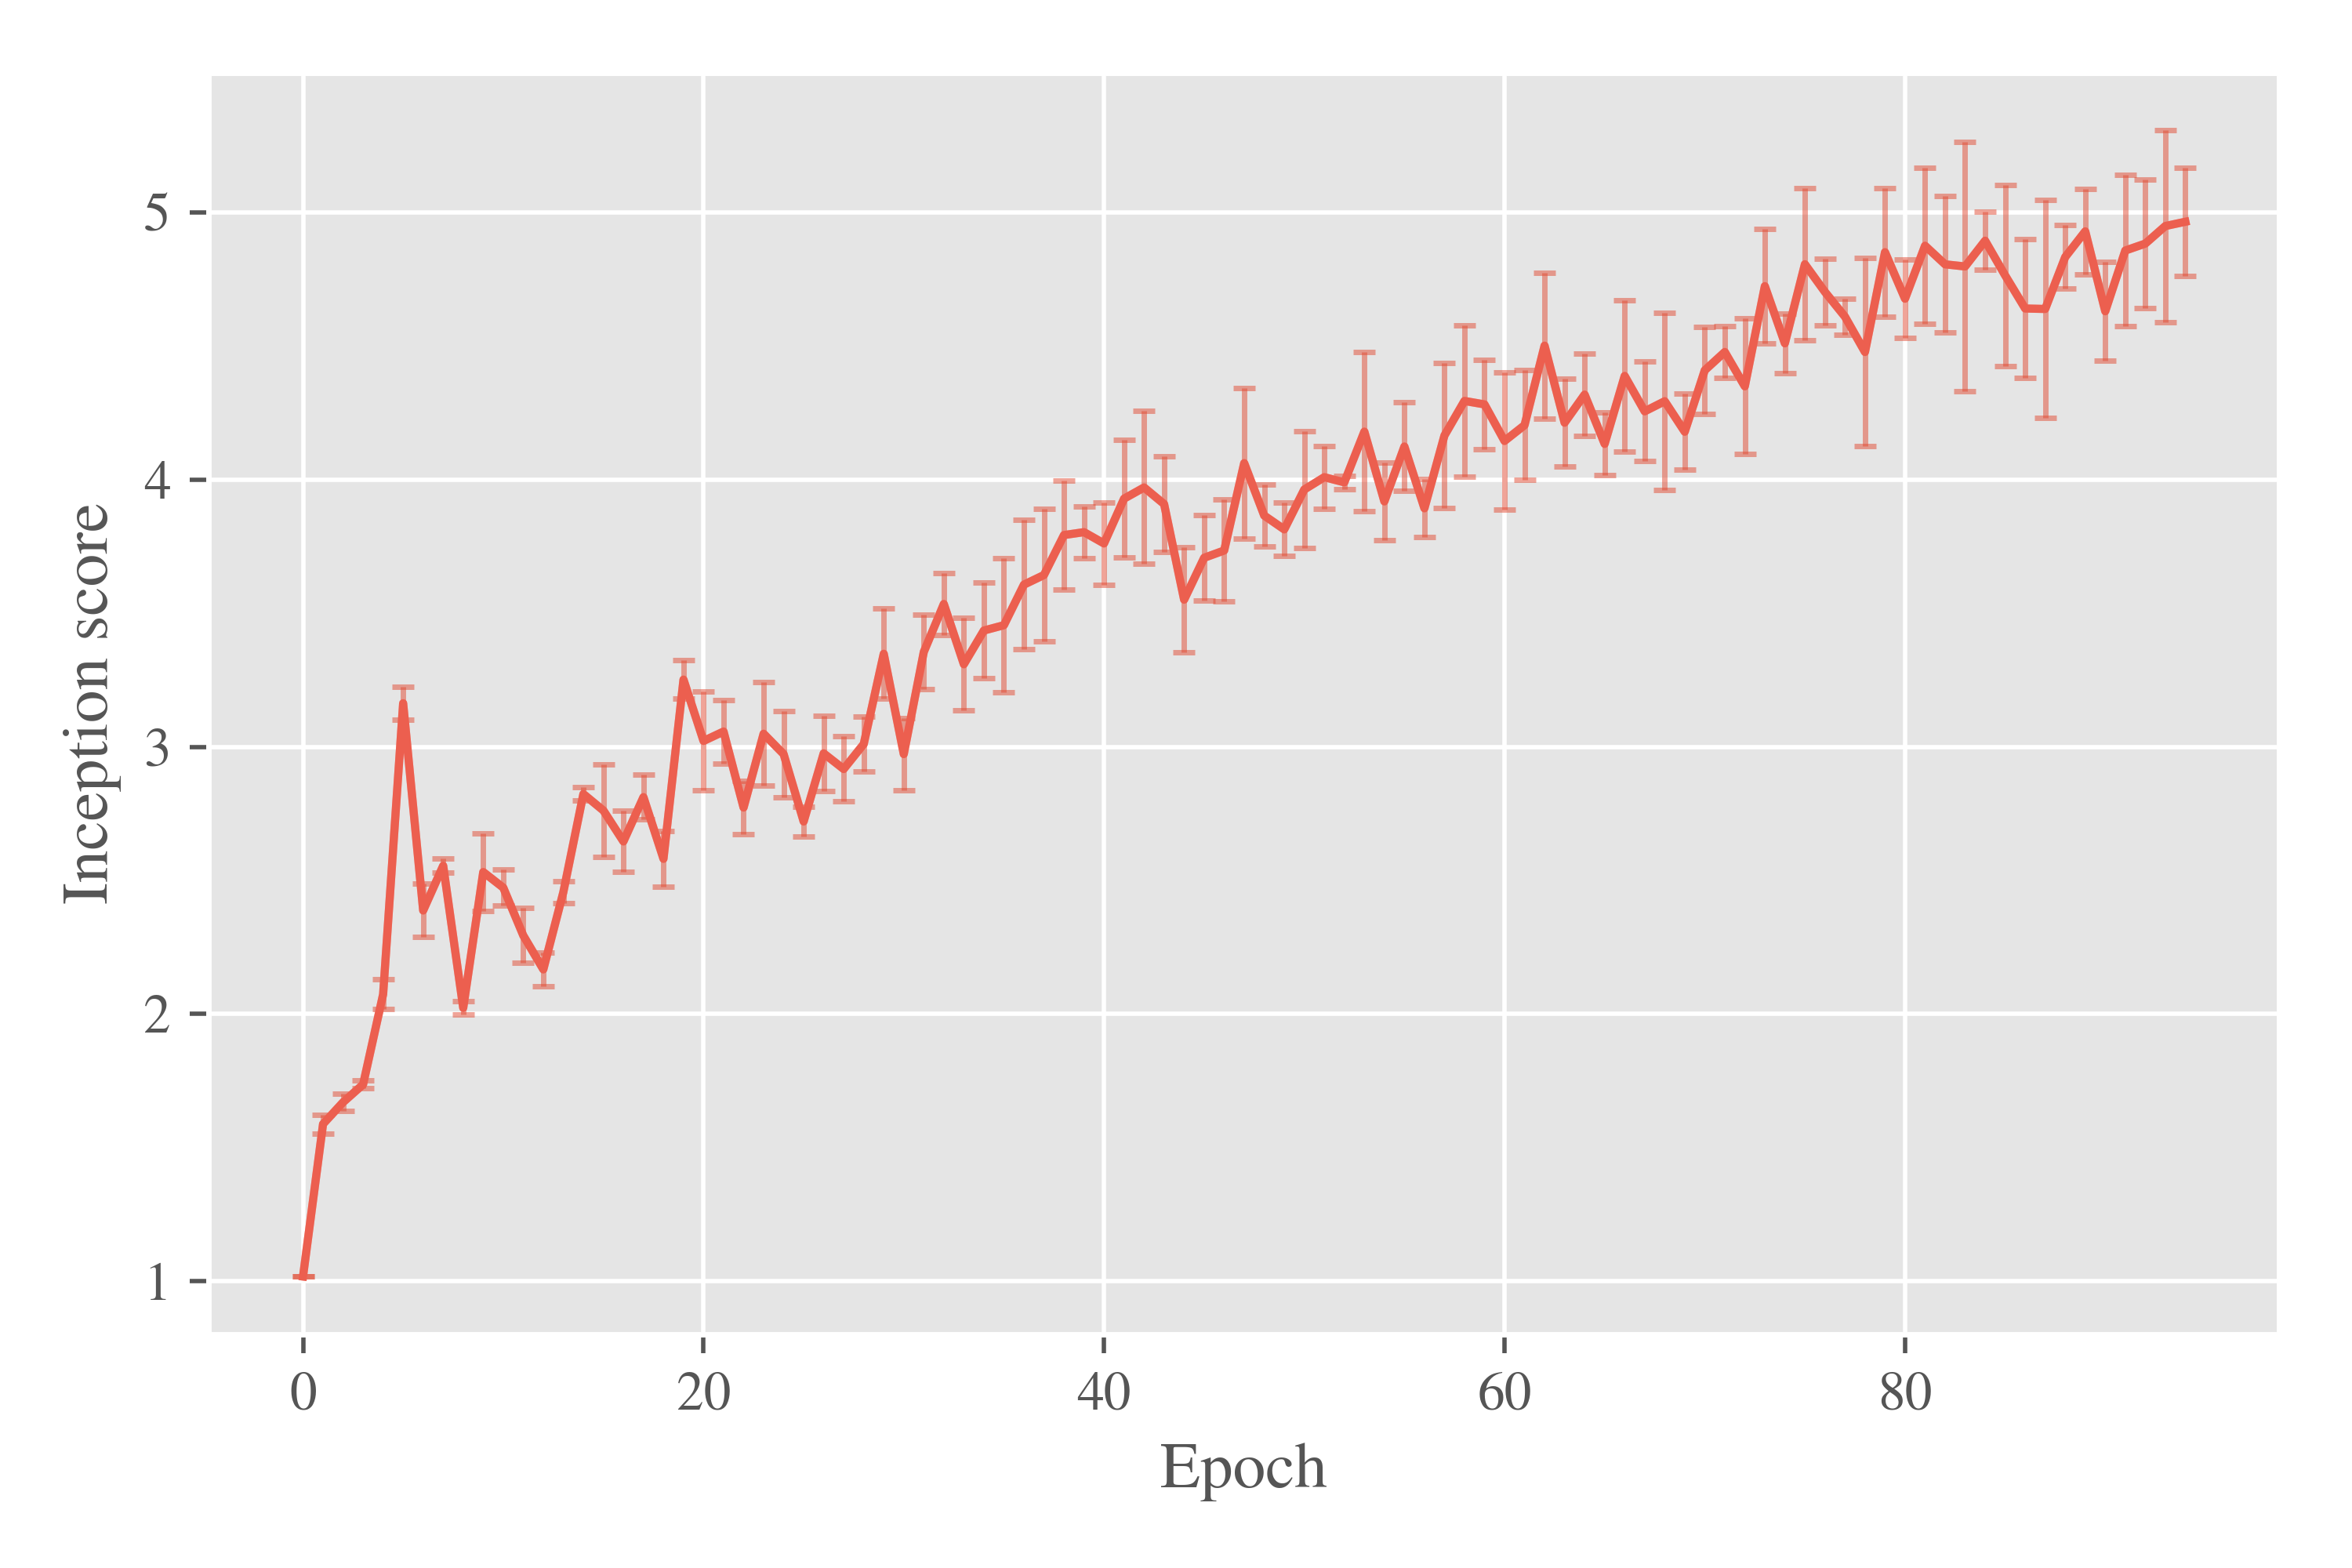
\includegraphics[width=\textwidth]{../code/results/figures/w-sn-dcgan_cifar10_is.png}
		\caption{Inception score}
		\label{fig:exp-w-sn-dcgan-is}
    \end{subfigure}
    \begin{subfigure}[t]{0.49\textwidth}
        \centering
        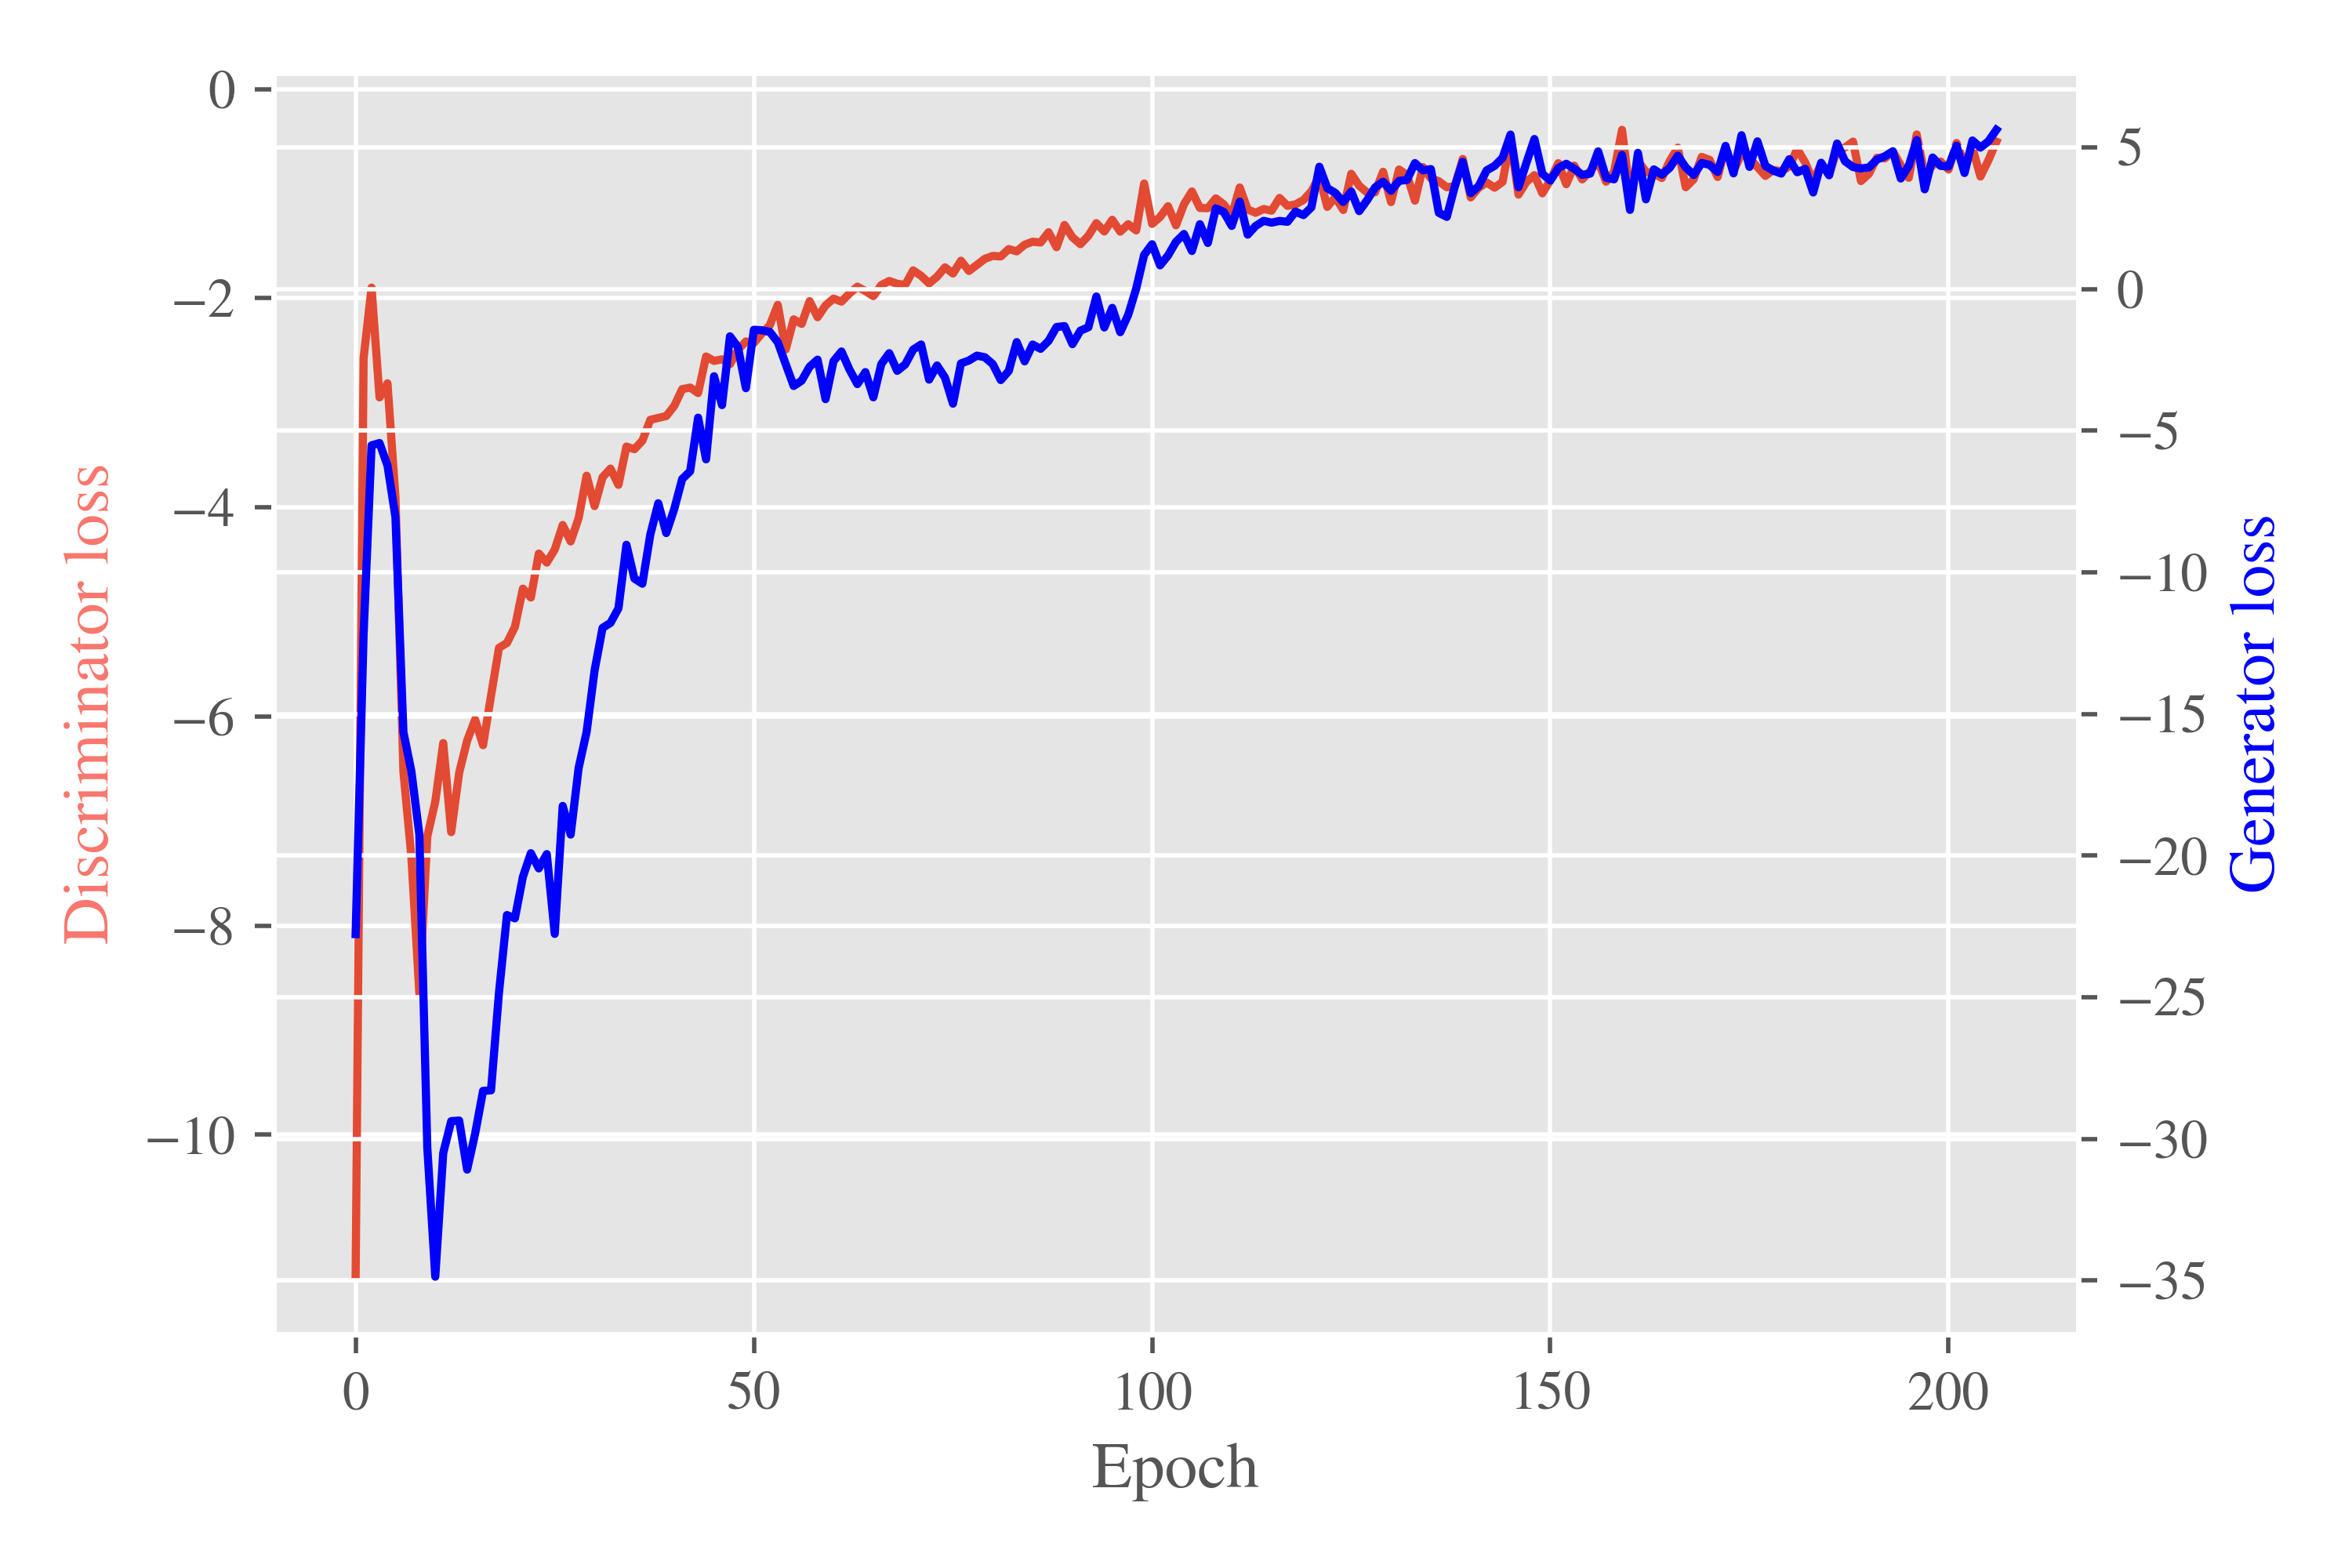
\includegraphics[width=\textwidth]{../code/results/figures/w-sn-dcgan_cifar10_losses.png}
		\caption{Losses}
		\label{fig:exp-w-sn-dcgan-losses}
    \end{subfigure}
    \caption{W-SN-DCGAN - training on CIFAR10 over 200 epochs.}
\end{figure}

